\documentclass[12pt]{article}

\usepackage[a4paper, includefoot,
left=3cm, right=1.5cm,
top=2cm, bottom=2cm,
headsep=1cm, footskip=1cm]{geometry}

\usepackage{amsmath,amssymb,amsthm,amscd,amsfonts}
\setlength{\parskip}{0.4cm}

\usepackage[utf8]{inputenc}
\usepackage[russian]{babel}
\usepackage{indentfirst}
\usepackage{graphicx}
\usepackage{wrapfig}
\usepackage{caption}
\usepackage{subfig}

\usepackage{import}
\usepackage{pgfplots}
\pgfplotsset{compat=1.9}

\usepackage{mathtext}
\usepackage{cmap}
\usepackage[T2A]{fontenc}
\usepackage{euscript}
\usepackage{mathdots}
\usepackage{epstopdf}


\newtheorem{theorem}{Теорерма}
%\newtheorem{corollary}[theorem]{Следствие}
\newtheorem{corollary}{Следствие}
\newtheorem{lemma}[theorem]{Лемма}
\newtheorem{observation}[theorem]{Observation}
\newtheorem{proposition}[theorem]{Предложение}
\newtheorem{definition}[theorem]{Определение}
\newtheorem{claim}[theorem]{Утверждение}
\newtheorem{fact}[theorem]{Факт}
\newtheorem{assumption}[theorem]{Предположение}
\newtheorem{alg}{Алгоритм}
\newtheorem{zam}{Замечание}

\newtheorem{example}{Пример}[section]

\newenvironment{Proof}{\par\noindent{\bf Доказательство.}}{\hfill$\scriptstyle\blacksquare$}
\newenvironment{ex}{\par\noindent{\bf Пример.}}{}
\newenvironment{pr1}{\par\noindent{\bf Дано:}}{}
\newenvironment{pr2}{\par\noindent{\bf Шаги:}}{}
\newenvironment{pr3}{\par\noindent{\bf Результат:}}{}

\DeclareMathOperator{\F}{\mathsf{F}}


\begin{document}
	
	
	\newgeometry{left=30mm, top=20mm, right=15mm, bottom=20mm, nohead, nofoot}

\begin{titlepage}
	\begin{center}
		
		\textbf{Санкт-Петербургский государственный университет\\Прикладная математика и информатика}
		
		\vspace{35mm}
	
		\textbf{\large  Отчет по научно-исследовательской работе } \\[8mm]
		\textbf{\large Замена непрерывных распределений на дискретные для применения на практике}\\ [8mm]
		\textbf{\large (семестр 8)}
		
		
		\vspace{20mm}

		\begin{flushright}
			{Выполнила:} \\
			Нагуманова Карина Ильнуровна, \\ группа 19.Б04-мм
		\end{flushright}
		\begin{flushright}
			{Научный руководитель:} \\
			к.ф.-м.н., доцент\\ Голяндина Нина Эдуардовна.\\ Кафедра статистического моделирования
		\end{flushright}
		
		\vfill 
		
		\textbf{Санкт-Петербург}
		\par{\textbf{2023}}
	\end{center}
\end{titlepage}

\restoregeometry
\addtocounter{page}{1}

	\tableofcontents
	\pagebreak
	
	\section{Введение}
	
	В практических задачах часто требуется заменить непрерывное распределение на
	дискретное с сохранением математического ожидания и дисперсии. Одним из методов
	нахождения такого распределения для аппроксимации нормального распределения является метод Свонсона. Однако в ряде областей, например, в нефтяной промышленности распределением, описывающим запасы нефти, общепринятым является логнормальное распределение. Соответственно, реальной задачей является аппроксимация логнормального распределения.
	
	С аппроксимируемыми случайными величинами производят сложение и умножение.
	Например, используем площадь дренирования пласта, среднюю чистую толщину и коэффициент извлечения углеводородов. При перемножении этих параметров получаем количество резервов нефти. Или зная запасы, параметры нефти и породы для всех залежей можно оценить профиль добычи нефти  с каждой залежи и суммарный профиль, оценить экономическую эффективность проекта, которая учитывает выручку, налоги, капитальные затраты, операционные затраты, оптимальные решения по проекту.
	Соответственно, возникает задача находить аппроксимацию суммы и произведения по аппроксимациям исходных случайных величин.
	
	Часто бывает на практике, что вместо настоящего распределения известны три его квантили, стандартно это 10-, 50- и 90-процентили. Задачей является нахождение по ним математического ожидания и дисперсии. Обычно задача решается построением весов для квантилей так, чтобы у полученного дискретного распределения были такие же математическое ожидание и дисперсия, как у исходного. Вообще говоря, иногда нужно, чтобы и более старшие моменты также аппроксимировались моментами построенного дискретного распределения с целью, чтобы для функций от распределений равенство математических ожиданий и дисперсий оставалось хотя бы приближенными.
	
	Структура работы следующая:\\
	В разделе 2 рассмотрен общий подход к трехточечной аппроксимации.\\
	В разделе 3 аппроксимация нормального распределения, вывод правила 30-40-30.\\
	В разделе 4 рассматривается аппроксимация логнормального распределения, условие аппроксимации и что делать, если это условие не выполняется. А также точность аппроксимации при применении правила 30-40-30 к логнормальному распределению.\\
	В разделе 5 алгоритм аппроксимации произведения двух логнормальных распределений.\\
	В разделе 6 алгоритм аппроксимации суммы двух логнормальных распределений.
	
	Работа этого семестра заключена в разделах 4.3, 4.4, 4.5, 6. В моей работе использовались статьи «Swanson's Swansong» \cite{Swansong} и «Uncertainties impacting reserves, revenue, and costs» \cite{Uncertainties}.
	
	Кроме этого были прочитаны следующие статьи:
	
	«Discretization, Simulation, and Swanson's (Inaccurate) Mean» \cite{Discretization}. В ней одна из частей исследования -- сравнение различных методов дискретизации непрерывных распределений, например таких, как Extended Person‐Tukey (EPT), McNamee‐Celona Shortcut (MCS), Extended Swanson‐Megill (ESM).
	
	Статья «Discretization, Simulation, and the Value of Information» \cite{Simulation}.
	Из нее понятно, что данный метод дискретизации значительно недооценивает среднее значение, дисперсию и асимметрию большинства распределений, особенно логнормального, где он широко используется. И что наилучшая дискретизация зависит от контекста решения, который мы не знаем заранее.
	
	А в статье «Performance Evaluation of Swanson’s Rule for the Case of Log-Normal Populations» \cite{Performance} проводится исследование оценки эффективности метода Свонсона и сравнение с использованием равных весов. Рассмотрены различные преимущества двух методов.
	
	\section{Условия аппроксимации в общем случае}
	
	Пусть дана случайная величина $\xi$ с математическим ожиданием $m$, дисперсией $s^{2}$ и функцией распределения $\F(x)$. Для неё заданы квантили $x_{\pi_{1}}$, $x_{\pi_{2}}$, $x_{\pi_{3}}$. Также есть случайная дискретная величина $\xi_{n}$ с математическим ожиданием $m_{n}$ и дисперсией $s^{2}_{n}$.
	\[\xi_{n}:\quad\begin{pmatrix} 
		x_{\pi_{1}}&x_{\pi_{2}}&x_{\pi_{3}}\\ 
		p_{1} &  p_{2}  & p_{3}
	\end{pmatrix}\]
	Мы хотим аппроксимировать распределение случайной величины $\xi$ дискретным распределением $\xi_{n}$.
	
	Нужно найти вероятности $p_{1}$, $p_{2}$, $p_{3}$ так, чтобы следующие равенства были верными.
	\begin{equation}
		p_{1} + p_{2} + p_{3} = 1, \label{1}
	\end{equation}
	\begin{equation}
		p_{1}x_{\pi_{1}} + p_{2}x_{\pi_{2}} + p_{3}x_{\pi_{3}} = m, \label{2}
	\end{equation}
	\begin{equation}
		p_{1} x_{\pi_{1}}^{2} + p_{2} x_{\pi_{2}}^{2} + p_{3} x_{\pi_{3}}^{2} - m^{2} = s^{2}. \label{3}
	\end{equation}
	
	Запишем уравнения \eqref{1}"---\eqref{3} в матричной форме следующим образом
	\[\begin{pmatrix} 
		1&1&1\\ 
		x_{\pi_{1}} &  x_{\pi_{2}}  & x_{\pi_{3}} \\ 
		x_{\pi_{1}}^2~~&x_{\pi_{2}}^2  &x_{\pi_{3}}^2
	\end{pmatrix}
	\begin{pmatrix}p_{1}\\p_{2}\\ p_{3}\end{pmatrix}= \begin{pmatrix}1\\m\\m^{2}+s^{2}\end{pmatrix}.\]
	
	Теперь введём более изящную форму, которая подчёркивает связь вероятностей с формой распределения путём нормализации математического ожидания и дисперсии.
	
	
	\begin{proposition}\label{pr1}
		Пусть верно 
		\begin{equation}
			\begin{pmatrix} 
				1&1&1\\ 
				\tilde{x}_{\pi_{1}}~~ &  \tilde{x}_{\pi_{2}}~~  & \tilde{x}_{\pi_{3}} \\ 
				\tilde{x}_{\pi_{1}}^{2}~~&\tilde{x}_{\pi_{2}}^{2}~~  &\tilde{x}_{\pi_{3}}^{2}
			\end{pmatrix}
			\begin{pmatrix}p_{1}\\p_{2}\\ p_{3}\end{pmatrix}= \begin{pmatrix}1\\0\\1 \end{pmatrix},\label{4}
		\end{equation}
		где $\tilde{x}_{\pi_{i}} = \tilde{\F}^{-1}(\pi_{i})$, $\tilde{\F}(y)$ "--- функция распределения $\displaystyle{\eta = \frac{\xi-m}{s}}$. Тогда $m=m_{n}$ и $s^{2} = s_{n}^{2}$.
	\end{proposition}
	\begin{Proof}
		\begin{align*}
			\mathsf{P}(\xi \leq x_{\pi_{i}}) &= \pi_{i},\\
			\mathsf{P}\left(\frac{\xi-m}{s}\leq \frac{x_{\pi_{i}}-m}{s}\right) &=  \tilde{\F}\left(\frac{x_{\pi_{i}}-m}{s}\right)=\pi_{i},
		\end{align*}
		$\xi$ нормализуется так, чтобы иметь нулевое математическое ожидание и единичную дисперсию.
		Имеем $x_{\pi_{i}} = m+s\tilde{\F}^{-1}(\pi_{i})$, обозначим
		\begin{equation}
			\tilde{x}_{\pi_{i}} = \dfrac{x_{\pi_{i}}-m}{s}=\tilde{\F}^{-1}(\pi_{i}). \label{5}
		\end{equation}
		Предположим, что $m=m_{n}$ и $s^{2} = s_{n}^{2}$, и получим систему \eqref{4}.
		Для этого подставим \eqref{5} в уравнение \eqref{2}, получаем
		\begin{equation*}
			m(p_{1} + p_{2} + p_{3})+s(p_{1}\tilde{x}_{\pi_1}+p_{2}\tilde{x}_{\pi_{2}}+p_{3}\tilde{x}_{\pi_{3}})=m.
		\end{equation*}
		Используя уравнение \eqref{1}, получаем
		\begin{equation*}
			s(p_{1}\tilde{x}_{\pi_1}+p_{2}\tilde{x}_{\pi_{2}}+p_{3}\tilde{x}_{\pi_{3}})=0.
		\end{equation*}
		Так как $s \neq 0$, то можно разделить на $s$, тогда получаем
		\begin{equation*}
			p_{1}\tilde{x}_{\pi_1}+p_{2}\tilde{x}_{\pi_{2}}+p_{3}\tilde{x}_{\pi_{3}}=0.
		\end{equation*}
		Теперь подставим \eqref{5} в уравнение \eqref{3}, получаем
		\begin{equation*}
			p_{1}(m+s\tilde{x}_{\pi_{1}})^{2}+p_{2}(m+s\tilde{x}_{\pi_{2}})^{2}+p_{3}(m+s\tilde{x}_{\pi_{3}})^{2} - m^{2} = s^{2},
		\end{equation*}
		\begin{equation*}
			p_{1}\tilde{x}_{\pi_{1}}^{2}+p_{2}\tilde{x}_{\pi_{2}}^{2}+p_{3}\tilde{x}_{\pi_{3}}^{2} = 1.
		\end{equation*}
		Получившиеся уравнения в матричной форме
		\begin{equation}
			\begin{pmatrix} 
				1&1&1\\ 
				\tilde{x}_{\pi_{1}}~~ &  \tilde{x}_{\pi_{2}}~~  & \tilde{x}_{\pi_{3}} \\ 
				\tilde{x}_{\pi_{1}}^{2}~~&\tilde{x}_{\pi_{2}}^{2}~~  &\tilde{x}_{\pi_{3}}^{2}
			\end{pmatrix}
			\begin{pmatrix}p_{1}\\p_{2}\\ p_{3}\end{pmatrix}= \begin{pmatrix}1\\0\\1 \end{pmatrix}. \label{6}
		\end{equation}
	\end{Proof}
	
	\section{Аппроксимация нормального распределения}
	В общем случае вероятности $p_{1}, p_{2}, p_{3}$ будут зависеть от математического ожидания и дисперсии, но если $\xi\sim N(\mu, \sigma) $ имеет нормальное распределение, то
	$\eta = \dfrac{\xi-m}{s}$ имеет нормальное стандартное распределение, которое не зависит ни от $\mu$, ни от $\sigma$.
	
	\begin{proposition}\label{pr7}
		$\xi\sim N(\mu, \sigma)$, пусть верно 
		\begin{equation}
			\begin{cases}
				p_{\pi} = \displaystyle{\frac{\delta}{2}},\\ 
				p_{0.5}=1-\delta , \\ 
				p_{1-\pi}=\displaystyle{\frac{\delta}{2}}.
			\end{cases}\label{7}
		\end{equation}
		где $\delta  = \displaystyle{\frac{1}{\Phi ^{-1}(\pi)^{2}}}$. Тогда $m=m_{n}$ и $s^{2} = s_{n}^{2}$.
	\end{proposition}
	\begin{proof}
		Предположим, что $m=m_{n}$ и $s^{2} = s_{n}^{2}$, и получим систему \eqref{7}.
		
		$\Phi (y) = \mathsf{P}(\eta = \dfrac{\xi-m}{s}\leq y)$ "--- функция распределения стандартного нормального распределения, тогда система \eqref{6} записывается как
		\begin{equation}
			\begin{pmatrix} 1&1&1\\ 
				\Phi^{-1}(\pi_{1})~~ &  \Phi ^{-1}(\pi_{2})~~  & \Phi ^{-1}(\pi_{3}) \\ 
				\Phi ^{-1}(\pi_{1})^{2}~~&\Phi ^{-1}(\pi_{2})^{2}~~  &\Phi ^{-1}(\pi_{3})^{2}
			\end{pmatrix}
			\begin{pmatrix}p_{1}\\p_{2}\\ p_{3}\end{pmatrix}= \begin{pmatrix}1\\0\\1\end{pmatrix}. \label{8}
		\end{equation}
		В частном случае симметричных квантилей вида $\pi$, 0.5, $1-\pi$ получаем $\Phi ^{-1}(\pi ) = -\Phi ^{-1}(1-\pi )$, $\Phi ^{-1}(0.5) = 0$, тогда система \eqref{8} упрощается до
		\begin{equation*}
			\begin{pmatrix} 1&1&1\\ 
				\Phi^{-1}(\pi)~~ &  0~~  & -\Phi ^{-1}(\pi) \\ 
				\Phi ^{-1}(\pi)^{2}~~& 0~~  &\Phi ^{-1}(\pi)^{2}
			\end{pmatrix} 
			\begin{pmatrix}p_{\pi}\\p_{0.5}\\ p_{1-\pi}\end{pmatrix}= \begin{pmatrix}1\\0\\1\end{pmatrix}.
		\end{equation*}
		
		\begin{equation}
			\begin{cases}
				p_{\pi}+p_{0.5}+p_{1-\pi} =1,\\ 
				(p_{\pi}-p_{1-\pi})\Phi ^{-1}(\pi) =0,\\ 
				(p_{\pi}+p_{1-\pi})\Phi ^{-1}(\pi)^{2}=1.
			\end{cases}\label{9}
		\end{equation}
		Обозначим $\delta  = \displaystyle{\frac{1}{\Phi ^{-1}(\pi)^{2}}}$, тогда из системы \eqref{9} получим систему \eqref{7}.
	\end{proof}
	
	
	Рассмотрим случай $\pi = 0.1$, имеем $\Phi ^{-1}(0.1) = -\Phi ^{-1}(0.9) \approx  -1.28$, $\Phi ^{-1}(0.5) = 0$, из уравнений системы \eqref{9} находим значения $p_{1}$, $p_{2}$, $p_{3}$.
	\begin{equation*}
		\begin{cases}
			p_{1}\approx 0.305, \\ 
			p_{2}\approx 0.390,  \\ 
			p_{3}\approx 0.305.
		\end{cases}
	\end{equation*}
	Эти вероятности примерно равны 0.3, 0.4, 0.3, поэтому это правило называют правилом 30-40-30 или \textbf{правилом Свонсона}.
	
	\section{Аппроксимация логнормального распределения}
	Пусть случайная величина $\eta$ имеет логнормальное распределение, тогда cлучайная величина $\xi = \ln(\eta)$ имеет нормальное распределение, $\xi \sim N(\mu, \sigma)$. И поэтому для нее можно использовать формулы, полученные в предыдущих разделах.
	
	\subsection{Способ нахождения вероятностей через математическое ожидание и дисперсию нормального распределения}
	Заметим, что если
	$x_{\pi_{1}}, x_{\pi_{2}}, x_{\pi_{3}}$ "--- квантили логнормального распределения, то $\ln(x_{\pi_{1}})$, $\ln(x_{\pi_{2}})$, $\ln(x_{\pi_{3}})$ "--- квантили нормального распределения. Можно взять эти квантили и использовать в способе нахождения вероятностей для нормального распределения. 
	
	Имеем следующий алгоритм.
	
	\begin{alg}\label{al1}
		\begin{pr1}
			квантили $x_{\pi_{1}}, x_{\pi_{2}}, x_{\pi_{3}}$ логнормальной случайной величины $\eta$, $\ln(\eta) \sim N(\mu, \sigma)$.
		\end{pr1}
		
		\begin{pr2}\end{pr2}
		\begin{enumerate}
			\item Вычисляем значения мат. ожидания $m$ и дисперсии $d$ случайной величины $\eta$, используя известные $x_{\pi_{1}}, x_{\pi_{2}}, x_{\pi_{3}}$.
			\item Выражаем параметры $\mu$ и $\sigma$ мат. ожидание и дисперсию соответствующего нормального распределения через параметры $m$ и $d$ логнормального распределения, используя следующие формулы
			\begin{equation}
				m = \exp(\mu+\frac{\sigma ^{2}}{2}),
			\end{equation} \label{10}
			\begin{equation}
				s^{2} = m^{2}[\exp(\sigma^{2})-1].
			\end{equation} \label{11}
			Заметим, что математическое ожидание логнормально распределенной случайной величины всегда положительное.
			\item С помощью системы \eqref{7} находим значения вероятностей $p_{1}$, $p_{2}$, $p_{3}$.
		\end{enumerate}
		\begin{pr3}\end{pr3} вероятности $p_{1}$, $p_{2}$, $p_{3}$ для $x_{\pi_{1}}, x_{\pi_{2}}, x_{\pi_{3}}$ случайной величины $\xi_{n}$.
		
	\end{alg}
	
	\begin{ex}
		Пусть у нас есть логнормальная случайная величина с $m = 2$, $s^{2} = 0.78125$.
		Значения квантилей $x_{10} = 1$, $x_{50} = 2$, $x_{90} = 3$.
		
		По данным формулам можно найти параметры соответствующего нормального распределения.
		\[\mu=0.69314,\] 
		\[\sigma=0.42863.\]
		Теперь можно найти значения $p_{1}$, $p_{2}$, $p_{3}$.
		\[p_{10}= 0.371243,\]
		\[p_{50}= 0.282992,\]
		\[p_{90}= 0.345764.\]
	\end{ex}
	\subsection{Непосредственная аппроксимация логнормального распределения}
	
	Есть другой способ нахождения результата, полученного в разделе 4.1. Можно не переходить к нормальному распределению, а сразу вычислять вероятности для квантилей логнормального распределения.
	
	Сначала найдём $\tilde{\F}(y)$ в терминах параметров распределения, затем найдём $\tilde{\F}^{-1}(p)$, чтобы использовать формулу \eqref{4}.
	
	\begin{proposition}\label{pr2}
		В терминах Предложения 1 функция $\tilde{\F}^{-1}(\pi)$ выражается через $\sigma$ как
		\begin{equation}
			\displaystyle{\tilde{\F}^{-1}(\pi) = y = \frac{\exp(\sigma\Phi^{-1}(\pi) - \frac{\sigma^{2} }{2})-1}{\sqrt{\exp(\sigma ^{2})-1}}}.
		\end{equation}\label{12}
	\end{proposition}
	\begin{Proof}
		\begin{align*}
			\tilde{\F}(y) &= \mathsf{P}\left(\eta\leq y \right) = \mathsf{P}\left(\frac{\xi-m}{s} \leq y \right)= \\
			&=\mathsf{P}(\log(\xi)\leq \log(m+sy))=\\
			&=\mathsf{P}\left( \frac{\log(\xi)-\mu}{\sigma}\leq \frac{\log(m+sy)-\mu}{\sigma} \right) =\\
			&=\Phi \left(\frac{\log(m+sy) - \mu}{\sigma}\right).
		\end{align*}
		Найдём $\log(m+sy)$, используя $m = e^{\mu +\frac{\sigma ^{2}}{2}}$ и $s = m\sqrt{e^{\sigma ^{2}}-1}$.
		\begin{equation*}
			m+sy = e^{\mu +\frac{\sigma ^{2}}{2}} + ye^{\mu +\frac{\sigma ^{2}}{2}}\sqrt{e^{\sigma ^{2}}-1} = e^{\mu +\frac{\sigma ^{2}}{2}}(1+y\sqrt{\exp(\sigma ^{2})-1}),
		\end{equation*}
		возьмем натуральный логарифм от обеих частей, получаем
		\begin{align*}
			\log(m+sy) &= \log(e^{\mu +\frac{\sigma ^{2}}{2}}(1+y\sqrt{\exp(\sigma ^{2})-1})) =\\
			&=\mu +\frac{\sigma ^{2}}{2} + \log(1+y\sqrt{\exp(\sigma ^{2})-1}),
		\end{align*}
		тогда
		\begin{equation*}
			\displaystyle{\frac{\log(m+sy)-\mu }{\sigma } = \frac{\sigma }{2} + \frac{\log(1+y\sqrt{\exp(\sigma ^{2})-1})}{\sigma}}.
		\end{equation*}
		
		То есть можно выразить
		\begin{equation*}
			\displaystyle{\tilde{\F}(y) = \Phi \left(\frac{\log(m+sy)-\mu }{\sigma }\right) = \Phi \left(\frac{\sigma }{2} + \frac{\log(1+y\sqrt{\exp(\sigma ^{2})-1})}{\sigma}\right)}.
		\end{equation*}
		
		Далее можно найти $\Phi^{-1}(\pi)$.
		\begin{equation*}
			\displaystyle{\Phi \left(\frac{\sigma }{2} + \frac{\log(1+y\sqrt{\exp(\sigma ^{2})-1})}{\sigma }\right) = \pi},
		\end{equation*}
		\begin{equation*}
			\displaystyle{\Phi^{-1}(\pi)=\frac{\sigma }{2} + \frac{\log(1+y\sqrt{\exp(\sigma ^{2})-1})}{\sigma}}.
		\end{equation*}
		
		Теперь можно найти $\log(1+y\sqrt{\exp(\sigma ^{2})-1})$.
		\begin{equation*}
			\displaystyle{\log(1+y\sqrt{\exp(\sigma ^{2})-1}) = \sigma\Phi^{-1}(\pi) - \frac{\sigma^{2} }{2}},
		\end{equation*}
		\begin{equation*}
			1+y\sqrt{\exp(\sigma ^{2})-1} = \exp(\sigma\Phi^{-1}(\pi) - \frac{\sigma^{2} }{2}).
		\end{equation*}
		
		В итоге получаем
		\begin{equation*}
			\displaystyle{\tilde{\F}^{-1}(\pi) = y = \frac{\exp(\sigma\Phi^{-1}(\pi) - \frac{\sigma^{2} }{2})-1}{\sqrt{\exp(\sigma ^{2})-1}}}.
		\end{equation*}
	\end{Proof}
	
	\begin{proposition}\label{pr3}
		Параметр $\sigma$ для логнормального распределения выражается через значения квантилей, как
		\begin{equation}
			\displaystyle{\sigma = \dfrac{\log\left(\dfrac{x_{\pi_{2}}}{x_{\pi_{1}}}\right)}{\Phi ^{-1}(\pi_{2}) - \Phi ^{-1}(\pi_{1})}}.
		\end{equation} \label{13}
	\end{proposition}
	\begin{Proof}
		Покажем, что дисперсию логнормального распределения можно вычислить из отношения двух квантилей.
		\begin{equation*}
			\mathsf{P}(\xi\leq x_{\pi}) = \pi,
		\end{equation*}
		\begin{equation*}
			\displaystyle{\mathsf{P}\left(\frac{\log(\xi)-\mu }{\sigma }\leq \frac{\log(x_{\pi})-\mu}{\sigma}\right) = \pi}.
		\end{equation*}
		Следовательно,
		\begin{equation*}
			\displaystyle{\Phi \left(\frac{\log(x_{\pi})-\mu}{\sigma}\right)=\pi},
		\end{equation*}
		и тогда
		\begin{equation}
			\log(x_{\pi})=\mu + \sigma\Phi ^{-1}(\pi).
		\end{equation}
		С помощью двух квантилей мы можем исключить $\mu$ из соответствующих уравнений. Пусть есть $\pi_{1}$-ый и $\pi_{3}$-ый квантили со значениями $x_{\pi_{1}}$ и $x_{\pi_{3}}$.
		\begin{equation*}
			\log(x_{\pi_{1}}) = \mu + \sigma\Phi ^{-1}(\pi_{1}),
		\end{equation*}
		\begin{equation*}
			\log(x_{\pi_{3}}) = \mu + \sigma\Phi ^{-1}(\pi_{3}).
		\end{equation*}
		Вычтем из второго уравнения первое, получаем
		\begin{equation*}
			\log\left(\frac{x_{\pi_{3}}}{x_{\pi_{1}}}\right) = \sigma(\Phi ^{-1}(\pi_{3})-\Phi ^{-1}(\pi_{1})).
		\end{equation*}
		И в итоге получаем
		\begin{equation*}
			\displaystyle{\sigma = \dfrac{\log\left(\dfrac{x_{\pi_{2}}}{x_{\pi_{1}}}\right)}{\Phi ^{-1}(\pi_{2}) - \Phi ^{-1}(\pi_{1})}}.
		\end{equation*}
	\end{Proof}
	
	\begin{alg}\label{al2}
		\begin{pr1}
			квантили $x_{\pi_{1}}, x_{\pi_{2}}, x_{\pi_{3}}$ логнормальной случайной величины $\eta$, $\ln(\eta) \sim N(\mu, \sigma)$.
		\end{pr1}
		
		\begin{pr2}\end{pr2}
		\begin{enumerate}
			\item Выражаем параметр $\sigma$ из отношения $x_{\pi_{3}}$ к $x_{\pi_{1}}$, используя формулу (13).
			\item Вычисляем значения $\tilde{\F}^{-1}(\pi)$ для случайной величины $\eta$ по формуле (12).
			\item С помощью системы \eqref{4} находим значения вероятностей $p_{1}$, $p_{2}$, $p_{3}$.
		\end{enumerate}
		\begin{pr3}\end{pr3} вероятности $p_{1}$, $p_{2}$, $p_{3}$ для $x_{\pi_{1}}, x_{\pi_{2}}, x_{\pi_{3}}$ случайной величины $\xi_{n}$.
		
	\end{alg}
	
	\begin{zam}
		Результаты Алгоритмов 1 и 2 совпадают.
	\end{zam}
	
	\begin{ex}
		
		Посчитаем пример для $\frac{x_{90}}{x_{10}}=3$. По формулам из этого раздела получаeм
		
		\[\sigma = \frac{\log(\frac{x_{90}}{x_{10}})}{\phi ^{-1}(0,9)-\phi ^{-1}(0,1)}\approx 0.428626,\]
		
		\[\mathsf{\tilde{F}}^{-1}(p)= \frac{\exp(\sigma \phi ^{-1}(p)-\frac{\sigma ^{2}}{2})-1}{\sqrt{\exp(\sigma ^{2})-1}}\].
		\[\mathsf{\tilde{F}}^{-1}(0.9) \approx 1.2915826424,\]
		\[\mathsf{\tilde{F}}^{-1}(0.1)  \approx -1.0539640761,\]
		\[\mathsf{\tilde{F}}^{-1}(0.5)  \approx -0.1954343914.\]
		
		Из системы (4) находим вероятности $p_{10}$, $p_{50}$, $p_{90}$.
		\[p_{10}= 0.371243,\]
		\[p_{50}= 0.282992,\]
		\[p_{90}= 0.345764.\]
		
	\end{ex}	
	
	\subsection{Условие на параметры для нахождения весов при аппроксимации логнормального распределения }
	
	Мы рассмотрели способы вычисления вероятностей для квантилей при аппроксимации логнормального распределения. Но эти вероятности находятся не при любом $\sigma$. Выясним, какое должно быть ограничение на этот параметр.
	\begin{proposition}
		Положительные вероятности $p_{1}$, $p_{2}$, $p_{3}$ для аппроксимации логнормальной случайной величины $\eta$ с квантилями вида $x_{\pi}$, $x_{0.5}$, $x_{1-\pi}$ существуют только при условии \[\exp(\sigma^{2})+\exp(-\sigma^{2})-\exp\left( \Phi^{-1}(\pi)\sigma-\dfrac{\sigma^{2}}{2}\right) -\exp\left( \Phi^{-1}(1-\pi)\sigma-\dfrac{\sigma^{2}}{2}\right) \leq 0,\]
	\end{proposition}
	\begin{Proof}
		\begin{equation*}
			\ln(\eta) \sim N(\mu, \sigma^{2}), \quad\quad \tilde{\F}(y) = \mathsf{P}\left(\eta\leq y \right).
		\end{equation*}
		С помощью формулы (12) найдем $\displaystyle{\tilde{\F}^{-1}(\pi_{i})}$ и сделаем следующие обозначения
		\[\tilde{\F}^{-1}(\pi) = t_{1}, \quad\quad\quad \tilde{\F}^{-1}(0.5) = t_{2}, \quad\quad\quad \tilde{\F}^{-1}(1-\pi) = t_{3}.\]
		Теперь рассмотрим систему \eqref{6}, запишем ее через $t_{1}$, $t_{2}$, $t_{3}$ и выразим вероятности $p_{1}$, $p_{2}$, $p_{3}$.
		\[p_{2}(t_{2}-t_{3})=p_{1}(t_{3}-t_{1})-t_{3},\]
		\[p_{1}(t_{1}^{2}-t_{3}^{2}) + p_{2}(t_{2}^{2} - t_{3}^{2})=1-t_{3}^{2}.\]
		Тогда получаем
		\[p_{1}(t_{1}^{2}-t_{3}^{2}) + (t_{2}+t_{3})(p_{1}(t_{3}-t_{1})-t_{3})=1-t_{3}^{2},\]
		\[p_{1}(t_{1}-t_{3})(t_{1}-t_{2})=1+t_{2}t_{3}.\]
		\begin{align}
			p_{1} &= \dfrac{1+t_{2}t_{3}}{(t_{1}-t_{3})(t_{1}-t_{2})}, \label{15}\\
			p_{2} &= \dfrac{p_{1}(t_{3}-t_{1})-t_{3}}{t_{2}-t_{3}}=\dfrac{1+t_{1}t_{3}}{(t_{2}-t_{1})(t_{2}-t_{3})}, \label{16}\\
			p_{3} &= 1-p_{1}-p_{2}. \label{17}
		\end{align}
		
		Все вероятности должны быть положительными, подставим в формулы для вероятностей значения переменных $t_{1}$, $t_{2}$, $t_{3}$, которые ищутся по формуле (11).
		\[p_{1}=\dfrac{1+\dfrac{\left( \exp\left( -\dfrac{\sigma^{2}}{2}\right) -1\right) \left( \exp(\Phi^{-1}(1-\pi)\sigma-\dfrac{\sigma^{2}}{2})-1\right) }{\exp(\sigma^{2})-1}}{\dfrac{\exp\left( \Phi^{-1}(\pi)\sigma-\dfrac{\sigma^{2}}{2}\right) -\exp\left( \Phi^{-1}(1-\pi)\sigma-\dfrac{\sigma^{2}}{2}\right) }{\sqrt{\exp(\sigma^{2})-1}}\dfrac{\exp\left( \Phi^{-1}(\pi)\sigma-\dfrac{\sigma^{2}}{2}\right) -\exp\left( -\dfrac{\sigma^{2}}{2}\right) }{\sqrt{\exp(\sigma^{2})-1}}}=\]
		
		\[=\dfrac{\exp(\sigma^{2})+\exp(\Phi^{-1}(1-\pi)\sigma-\sigma^{2})-\exp(-\dfrac{\sigma^{2}}{2})-\exp(\Phi^{-1}(1-\pi)\sigma-\dfrac{\sigma^{2}}{2})}{\exp(\Phi^{-1}(0.1)*2\sigma-\sigma^{2})-\exp(\Phi^{-1}(\pi)\sigma-\sigma^{2})-\exp(-\sigma^{2})+\exp(\Phi^{-1}(1-\pi)\sigma-\sigma^{2})}.\]
		
		\[p_{2}=\dfrac{1+\dfrac{(\exp(\Phi^{-1}(\pi)\sigma-\dfrac{\sigma^{2}}{2})-1)(\exp(\Phi^{-1}(1-\pi)\sigma-\dfrac{\sigma^{2}}{2})-1)}{\exp(\sigma^{2})-1}}{\dfrac{\exp(-\dfrac{\sigma^{2}}{2})-\exp(\Phi^{-1}(\pi)\sigma-\dfrac{\sigma^{2}}{2})}{\sqrt{\exp(\sigma^{2})-1}}\dfrac{\exp(-\dfrac{\sigma^{2}}{2})-\exp(\Phi^{-1}(1-\pi)\sigma-\dfrac{\sigma^{2}}{2})}{\sqrt{\exp(\sigma^{2})-1}}}=\]
		
		\[=\dfrac{\exp(\sigma^{2})+\exp(-\sigma^{2})-\exp(\Phi^{-1}(\pi)\sigma-\dfrac{\sigma^{2}}{2})-\exp(\Phi^{-1}(1-\pi)\sigma-\dfrac{\sigma^{2}}{2})}{\exp(-\sigma^{2})-\exp(\Phi^{-1}(1-\pi)\sigma-\sigma^{2})-\exp(\Phi^{-1}(\pi)\sigma-\sigma^{2})+\exp(-\sigma^{2})}=\]
		
		\[=\dfrac{\exp(\sigma^{2})+\exp(-\sigma^{2})-\exp\left( \dfrac{\sigma^{2}}{2}\right)\left(\exp(\Phi^{-1}(\pi)\sigma)+\exp(-\Phi^{-1}(\pi)\sigma)\right) }{2\exp(-\sigma^{2})-\exp(-\sigma^{2})\left( \exp(-\Phi^{-1}(\pi)\sigma)+\exp(\Phi^{-1}(\pi)\sigma)\right) }.\]
		
		Вероятности $p_{1}$ и $p_{3}$ положительные при любом параметре $\sigma$. Рассмотрим знаменатель $p_{2}$.
		\[2\exp(-\sigma^{2})-\exp(-\sigma^{2})\left( \exp(-\Phi^{-1}(\pi)\sigma)+\exp(\Phi^{-1}(\pi)\sigma)\right)=\]
		\[=\exp(-\sigma^{2})(2- \exp(-\Phi^{-1}(\pi)\sigma)-\exp(\Phi^{-1}(\pi)\sigma))=\]
		\[=-\dfrac{\exp(-\sigma^{2})(\exp(\Phi^{-1}(\pi)\sigma)-1)^{2}}{\exp(\Phi^{-1}(\pi)\sigma)}.\]
		Числитель и знаменатель дроби положительные при любом значении параметра $\sigma$. Значит, весь знаменатель $p_{2}$ отрицательный. Из условия отрицательности числителя получаем следующее ограничение на $\sigma$.
		\[\exp(\sigma^{2})+\exp(-\sigma^{2})-\exp\left( \dfrac{\sigma^{2}}{2}\right)\left(\exp(\Phi^{-1}(\pi)\sigma)+\exp(-\Phi^{-1}(\pi)\sigma)\right) \leq 0.\]
	\end{Proof}
	
	
	Например, для $\pi=0.1$ получаем ограничение $\sigma\leq 0.6913$. 
	Посмотрим, какому коэффициенту асимметрии соответствует это значение $\sigma$.
	\[\gamma_{3} = \sqrt{\exp(\sigma^{2})-1}(\exp(\sigma^{2})+2),\]
	\[\gamma_{3} = 2.82778.\]
	
	Ограничение на $\sigma$ становится слабее при уменьшении значения $\pi$.
	
	Рассмотрим $\pi = 0.05$, получаем ограничение $\sigma \leq 1.04585$.
	\[\gamma_{3} = 7.02529.\]
	
	При уменьшении $\pi$ и фиксированной сигме то, что вычитается, растет и в какой-то момент становится больше уменьшаемого.
	
	
	\subsection{Варианты постановки задачи}
	
	\textbf{Задача:} имеются квантили $x_{\pi}$, $x_{0.5}$, $x_{1-\pi}$ логнормальной случайной величины $\eta$. Нужно уметь считать её математическое ожидание и дисперсию.
	
	Варианты решения задачи:
	\begin{enumerate}
		\item Не переходить к аппроксимации дискретной случайной величиной, а сразу же из двух уравнений вида (14), записанных для двух квантилей, найти значения параметров $\mu$ и $\sigma$ нормальной случайной величины $\ln(\eta)\sim N(\mu, \sigma)$. Далее по формулам (10) и (11) вычислить значения мат. ожидания $m$ и дисперсии $s^{2}$ случайной величины $\eta$.
		\item Перейти к трехточечной аппроксимации дискретной случайной величиной $\xi_{n}$, у которой мат. ожидание и дисперсия равны мат. ожиданию $m$ и дисперсии $s^{2}$ случайной величины $\xi$. И считать значения $m$ и $s$ через квантили $x_{\pi}$, $x_{0.5}$, $x_{1-\pi}$ и вероятности $p_{1}$, $p_{2}$, $p_{3}$.
		\item Если условие для положительных вероятностей не выполняется, можно воспринимать задачу не как поиск вероятностей для $\xi_{n}$, а как поиск коэффициентов для $x_{\pi}$, $x_{0.5}$, $x_{1-\pi}$ таких, чтобы параметры, полученные по формулам (2) и (3), были равны мат. ожиданию и дисперсии $\eta$. 
	\end{enumerate}
	
	\subsection{Точность аппроксимации}
	
	Предлагаемые методы аппроксимации логнормального распределения не работают при $\sigma \leq 0.6913$. На практике часто используют правило Свонсона 30-40-30 для аппроксимации логнормального распределения, поэтому посмотрим на точность 30-40-30. Особенно это важно при $\sigma \geq 0.6913$.
	
	\subsubsection{Неправильное использование правила 30-40-30}
	
	\begin{proposition}\label{pr5}
		Ошибка аппроксимации мат.ожидания логнормального распределения с помощью правила 30-40-30 равна
		\[\dfrac{\mid m_{1} - m_{2} \mid}{m_{1}} = \dfrac{\left|\exp\left(\dfrac{\sigma^{2}}{2}\right) - \dfrac{1}{2(\Phi^{-1}(0.1))^{2}}\left(\exp(\sigma\Phi^{-1}(0.1))-1 +\exp(\sigma\Phi^{-1}(0.9))\right) + 1\right|}{\exp\left(\dfrac{\sigma^{2}}{2}\right)}\]
		и не зависит от параметра $\mu$.
	\end{proposition}
	\begin{Proof}
		Выразим ошибку аппроксимации мат.ожидания логнормального распределения через параметры $\mu$ и $\sigma$.
		\[m_{1} = \exp\left(\mu+\dfrac{\sigma^{2}}{2}\right).\]
		Имеем следующие квантили
		\[x_{\pi} = \exp(\mu+\sigma\Phi^{-1}(0.1)),\]
		Точные значения вероятностей
		\[p_{1} = p_{3} = \dfrac{1}{2(\Phi^{-1}(0.1))^{2}},\]
		\[p_{2} = 1 - \dfrac{1}{(\Phi^{-1}(0.1))^{2}}.\]
		
		Тогда мат.ожидание аппроксимации равно
		\[m_{2} = \dfrac{1}{2(\Phi^{-1}(0.1))^{2}}\exp(\mu+\sigma\Phi^{-1}(0.1))+\]
		\[+\left(1 - \dfrac{1}{(\Phi^{-1}(0.1))^{2}}\right)\exp(\mu+\sigma\Phi^{-1}(0.5))+ \dfrac{1}{2(\Phi^{-1}(0.1))^{2}}\exp(\mu+\sigma\Phi^{-1}(0.9))=\]
		\[= \dfrac{1}{2(\Phi^{-1}(0.1))^{2}} \exp(\mu)(\exp(\sigma\Phi^{-1}(0.1))-1+\exp(\sigma\Phi^{-1}(0.9))) + \exp(\mu). \]
		
		Получили ошибку
		\[\dfrac{\left| m_{1} - m_{2} \right|}{m_{1}} = \]\[=\dfrac{\left| \exp\left(\mu+\dfrac{\sigma^{2}}{2}\right) - \dfrac{1}{2(\Phi^{-1}(0.1))^{2}} \exp(\mu)(\exp(\sigma\Phi^{-1}(0.1))-1 +\exp(\sigma\Phi^{-1}(0.9))) + \exp(\mu) \right|}{\exp\left(\mu+\dfrac{\sigma^{2}}{2}\right)}=\]
		\[=\dfrac{\left| \exp\left(\dfrac{\sigma^{2}}{2}\right) - \dfrac{1}{2(\Phi^{-1}(0.1))^{2}} (\exp(\sigma\Phi^{-1}(0.1))-1 +\exp(\sigma\Phi^{-1}(0.9))) + 1 \right|}{\exp\left(\dfrac{\sigma^{2}}{2}\right)}=\]
	\end{Proof}
	
	\begin{figure}[h]
		\begin{center}
			\begin{minipage}[h]{0.4\linewidth}
				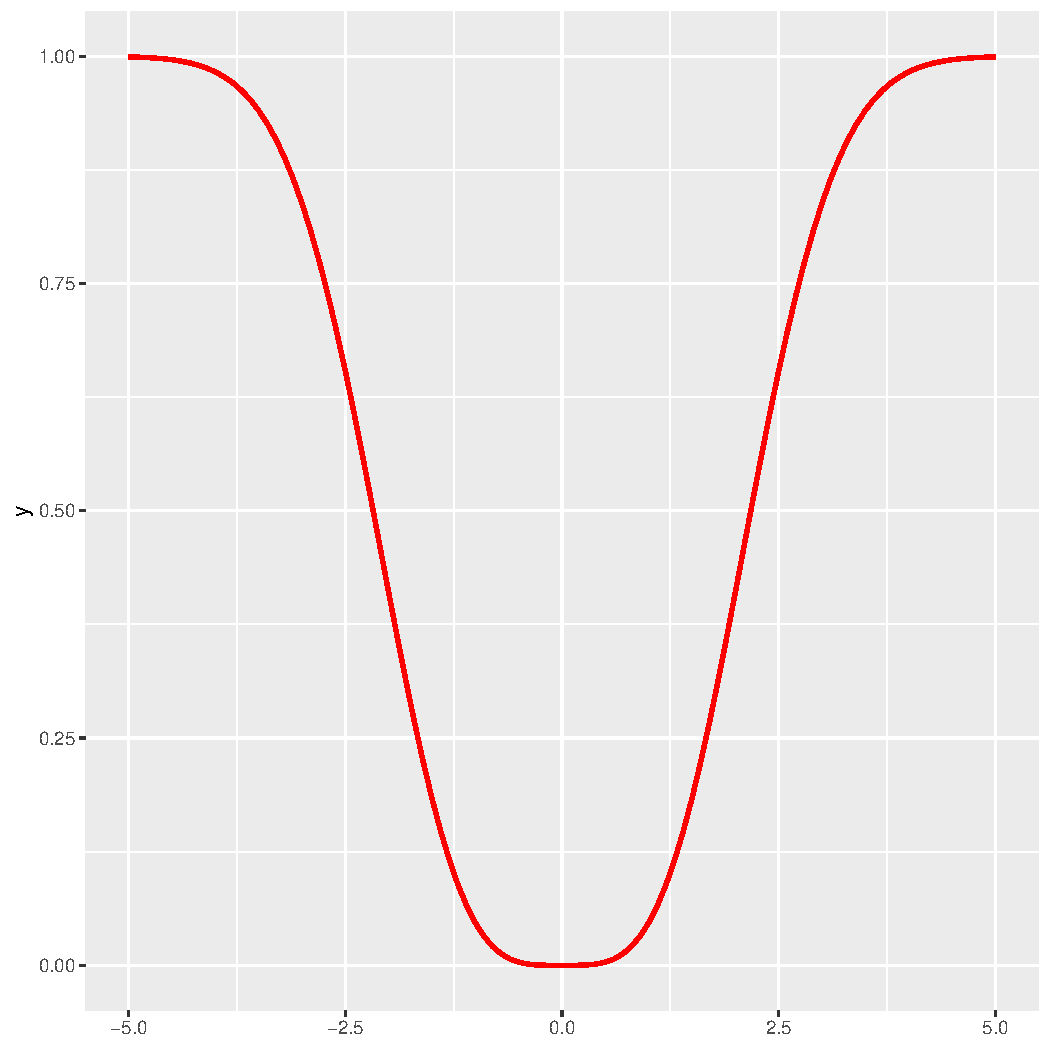
\includegraphics[width=1\linewidth]{ris4.pdf}
				\caption{Ошибка аппроксимации мат.ожидания.} %% подпись к рисунку
				\label{ris1} %% метка рисунка для ссылки на него
			\end{minipage}
			\hfill
			\begin{minipage}[h]{0.4\linewidth}
				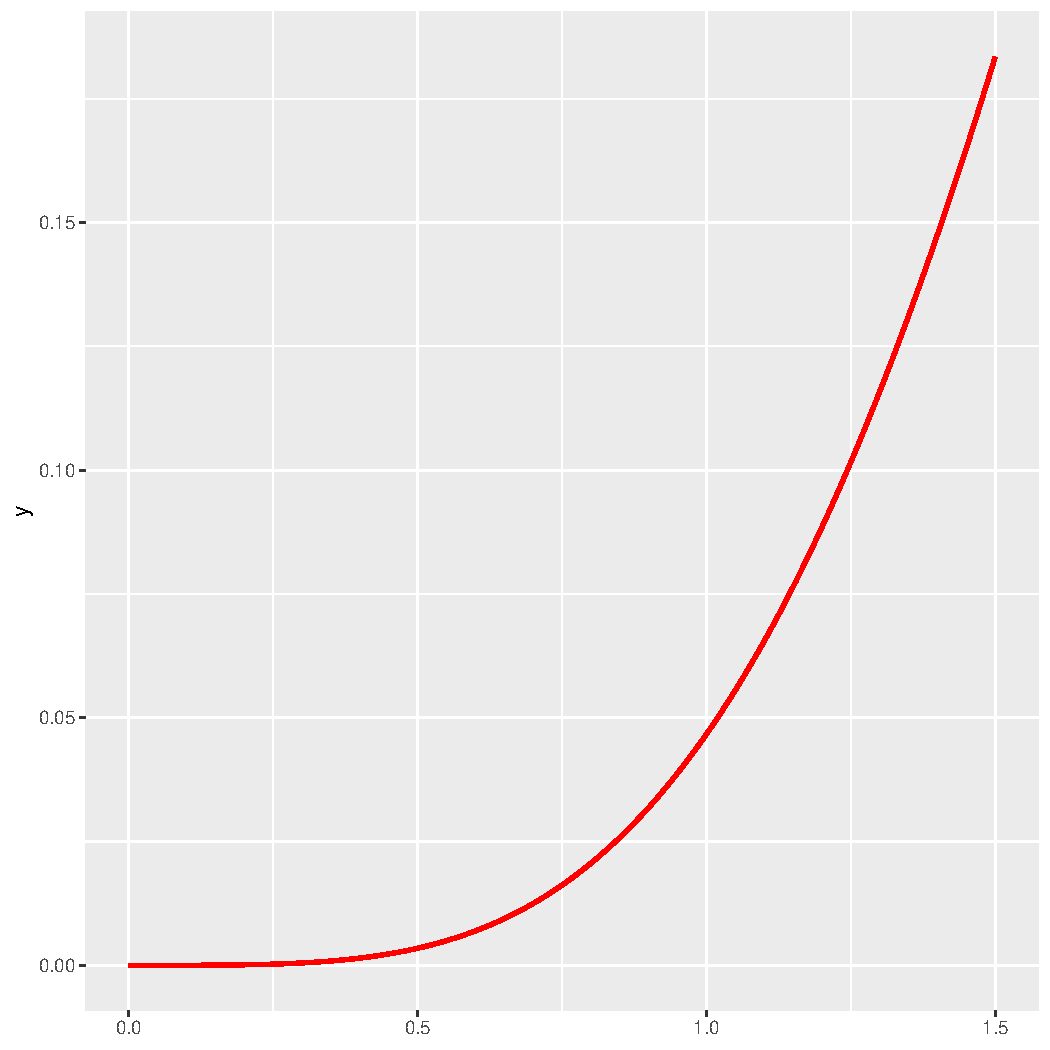
\includegraphics[width=1\linewidth]{ris1.pdf}
				\caption{Ошибка аппроксимации мат.ожидания, $\sigma\leq 1.5.$}
				\label{ris2}
			\end{minipage}
		\end{center}
	\end{figure}
	
	
	\begin{proposition}\label{pr6}
		Ошибка аппроксимации дисперсии логнормального распределения с помощью правила 30-40-30 равна
		\[\dfrac{\mid d_{1} - d_{2} \mid}{d_{1}} = \mid \exp(\sigma^{2})(\exp(\sigma^{2}-1)) - \dfrac{1}{2(\Phi^{-1}(0.1))^{2}}\exp(2\sigma\Phi^{-1}(0.1))-\]
		\[- \left(1 - \dfrac{1}{(\Phi^{-1}(0.1))^{2}}\right)\exp(2\sigma\Phi^{-1}(0.5))-\]
		\[-\dfrac{1}{2(\Phi^{-1}(0.1))^{2}}\exp(2\sigma\Phi^{-1}(0.9)) + m_{2}^{2}/2\mu\mid/\exp(\sigma^{2})(\exp(\sigma^{2}-1))\]
		
		и не зависит от параметра $\mu$.
	\end{proposition}
	\begin{Proof}
		Выразим аппроксимации дисперсии через параметры распределения.
		\[d_{1} = \exp(2\mu+\sigma^{2})(\exp(\sigma^{2}-1)).\]
		\[d_{2} = \dfrac{1}{2(\Phi^{-1}(0.1))^{2}}\exp(2\mu+2\sigma\Phi^{-1}(0.1))+ \]
		\[+\left(1 - \dfrac{1}{(\Phi^{-1}(0.1))^{2}}\right)\exp(2\mu+2\sigma\Phi^{-1}(0.5))+ \dfrac{1}{2(\Phi^{-1}(0.1))^{2}}\exp(2\mu+2\sigma\Phi^{-1}(0.9)) - m_{2}^{2}.\]
		
		Получили ошибку
		\[\dfrac{\mid d_{1} - d_{2} \mid}{d_{1}} = \mid \exp(2\mu+\sigma^{2})(\exp(\sigma^{2}-1)) - \dfrac{1}{2(\Phi^{-1}(0.1))^{2}}\exp(2\mu+2\sigma\Phi^{-1}(0.1))-\]
		\[- \left(1 - \dfrac{1}{(\Phi^{-1}(0.1))^{2}}\right)\exp(2\mu+2\sigma\Phi^{-1}(0.5))-\]
		\[-\dfrac{1}{2(\Phi^{-1}(0.1))^{2}}\exp(2\mu+2\sigma\Phi^{-1}(0.9)) + m_{2}^{2}\mid/\exp(2\mu+\sigma^{2})(\exp(\sigma^{2}-1))=\]
		\[=\mid \exp(\sigma^{2})(\exp(\sigma^{2}-1)) - \dfrac{1}{2(\Phi^{-1}(0.1))^{2}}\exp(2\sigma\Phi^{-1}(0.1))-\]
		\[- \left(1 - \dfrac{1}{(\Phi^{-1}(0.1))^{2}}\right)\exp(2\sigma\Phi^{-1}(0.5))-\]
		\[-\dfrac{1}{2(\Phi^{-1}(0.1))^{2}}\exp(2\sigma\Phi^{-1}(0.9)) + m_{2}^{2}/2\mu\mid/\exp(\sigma^{2})(\exp(\sigma^{2}-1)).\]
	\end{Proof}
	
	\begin{figure}[h]
		\begin{center}
			\begin{minipage}[h]{0.4\linewidth}
				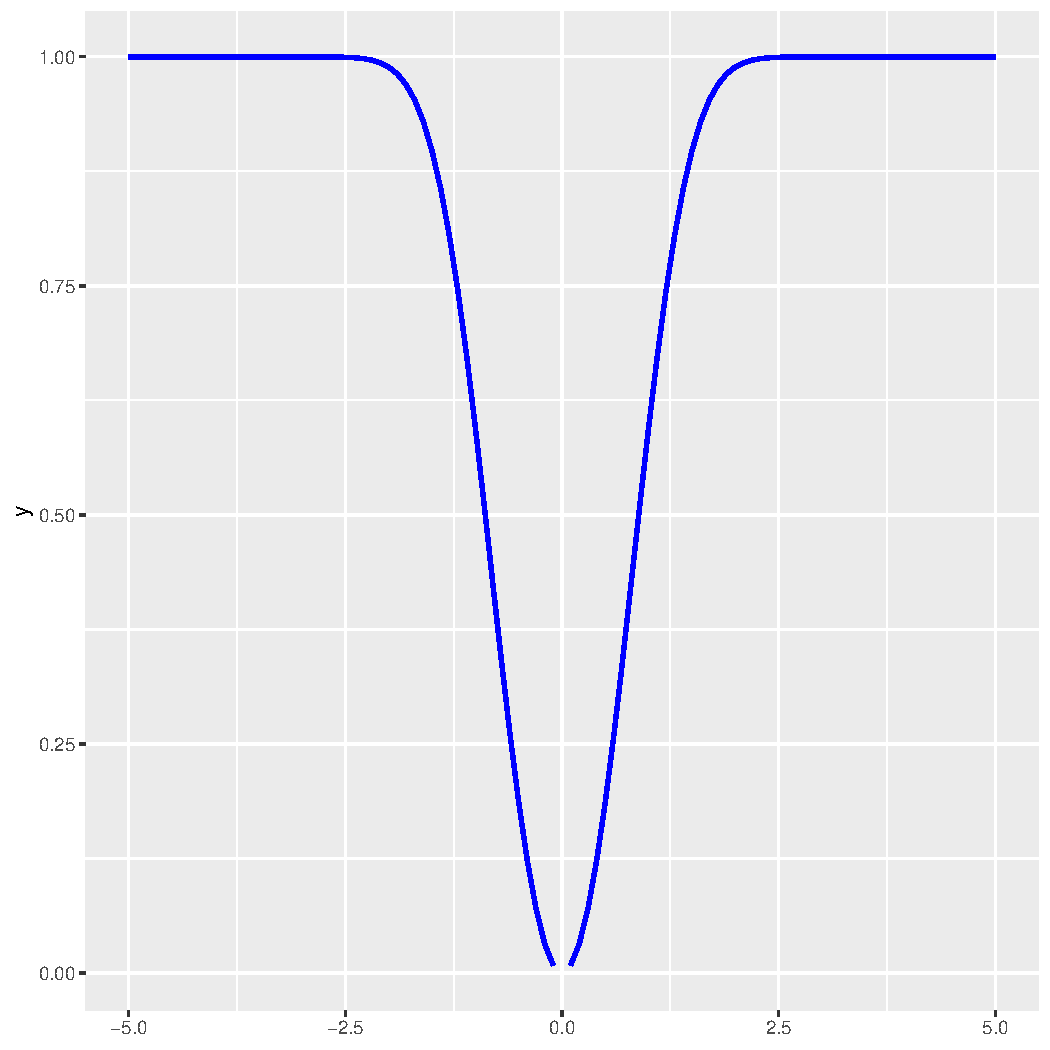
\includegraphics[width=1\linewidth]{ris2.pdf}
				\caption{Ошибка аппроксимации дисперсии.} %% подпись к рисунку
				\label{ris3} %% метка рисунка для ссылки на него
			\end{minipage}
			\hfill
			\begin{minipage}[h]{0.4\linewidth}
				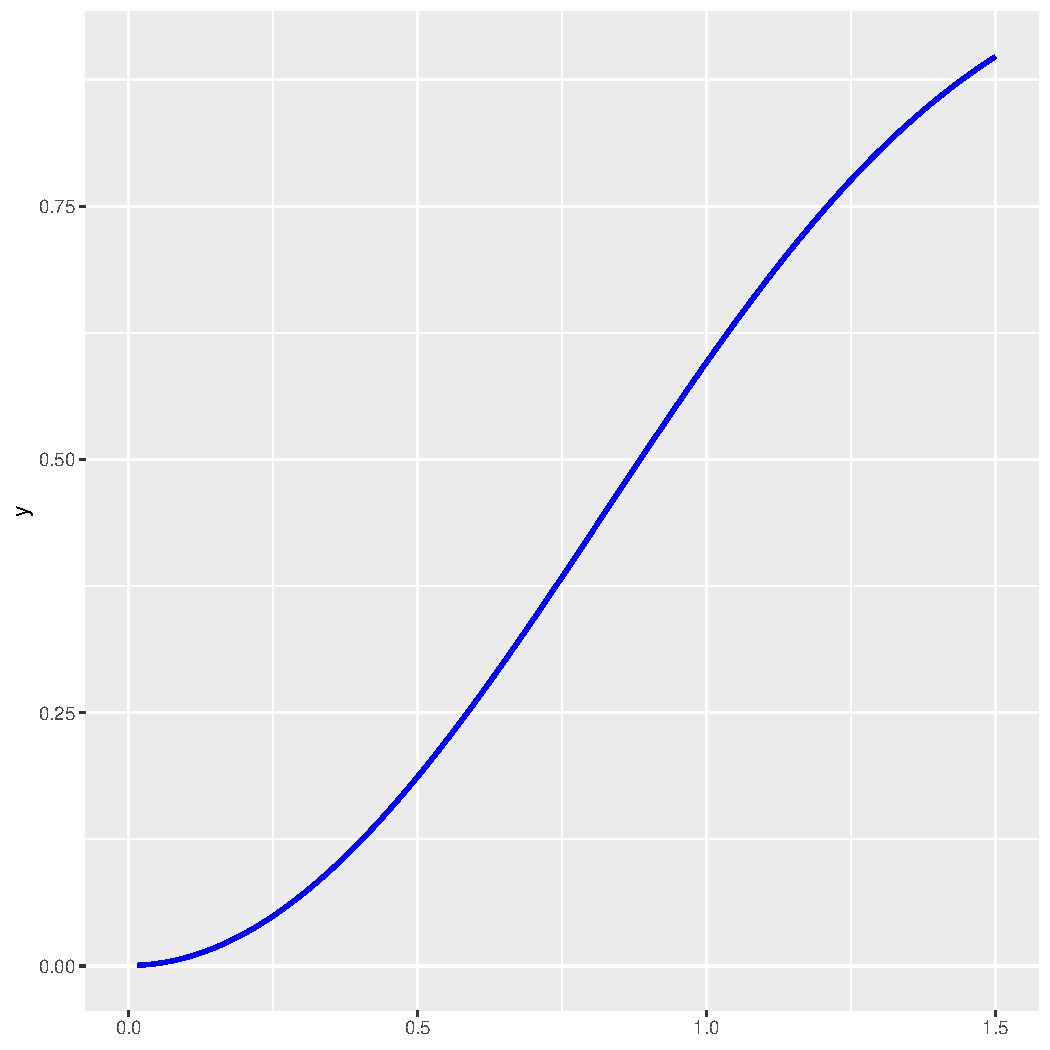
\includegraphics[width=1\linewidth]{ris3.pdf}
				\caption{Ошибка аппроксимации дисперсии, $\sigma\leq 1.5.$}
				\label{ris4}
			\end{minipage}
		\end{center}
	\end{figure}
	
	\section{Произведение двух логнормальных распределений}
	Нам доступен метод объединения любых логнормально распределенных случайных величин. Эта процедура применяется в нефтяной промышленности, она выполняется быстро и может быть выполнена вручную. Например, используем площадь дренирования пласта, среднюю чистую толщину и коэффициент извлечения углеводородов. При перемножении этих параметров получаем количество резервов нефти.
	
	Рассмотрим произведение любых двух логнормально распределенных случайных величин.
	\begin{equation*}
		\ln(\xi_{1}) \sim N(\mu_{1}, \sigma _{1}^{2}),
	\end{equation*}
	\begin{equation*}
		\ln(\xi_{2}) \sim N(\mu_{2}, \sigma _{2}^{2}).
	\end{equation*}
	
	Введем следующие обозначения:\\
	$x_{\pi}$, $x_{0.5}$, $x_{1-\pi}$ "--- квантили случайной величины $\xi_{1}$,\\
	$y_{\pi}$, $y_{0.5}$, $y_{1-\pi}$ "--- квантили случайной величины $\xi_{2}$.
	
	\begin{proposition}
		При перемножении квантилей $x_{\pi}$ и $y_{\pi}$ двух логнормальных случайных величин $\xi_{1}$ и $\xi_{2}$ получается квантиль случайной величины $\xi_{1}\xi_{2}$ вида $z_{q}$, где
		
		\begin{equation}
			q = \mathsf{P}(\xi_{1}\xi_{2}< x_{\pi}y_{\pi}) =\Phi\left(\frac{\Phi^{-1}(\pi)(\ln(x_{0.5})+\ln(y_{0.5})-\ln(x_{\pi})-\ln(y_{\pi}))}{\sqrt{(\ln(x_{0.5})-\ln(x_{\pi}))^{2}+(\ln(y_{0.5})-\ln(y_{\pi}))^{2}}}\right).
		\end{equation} 
	\end{proposition}
	\begin{Proof}
		Выразим параметры распределений $\mu_{1}$, $\mu_{2}$, $\sigma_{1}$, $\sigma_{2}$ через квантили.
		По определению квантиля $\mathsf{P}(\xi_{1}<x_{\pi}) = \pi$.
		
		Преобразуем эту вероятность так, чтобы ее можно было записать через функцию распределения стандартного нормального распределения, следующим образом:
		\begin{equation*}
			\mathsf{P}(\xi_{1}<x_{\pi}) = \mathsf{P}(\ln(\xi_{1})<\ln(x_{\pi})) = \mathsf{P}\left(\dfrac{\ln(\xi_{1})-\mu_{1}}{\sigma_{1}} < \frac{\ln(x_{\pi})-\mu_{1}}{\sigma_{1}}\right).
		\end{equation*}
		Так как $\xi_{1}$ распределена логнормально с параметрами $\mu_{1}$ и $\sigma_{1}^{2}$, то \[\dfrac{\ln(\xi_{1})-\mu_{1}}{\sigma_{1}} \sim N(0,1).\]
		
		Следовательно, можно записать логарифм квантиля, как:
		\begin{equation}
			\ln(x_{\pi})=\sigma_{1}\Phi^{-1}(\pi)+\mu_{1}.\label{12}
		\end{equation}
		
		Аналогично для $x_{50}$, получаем, что 
		\begin{equation}
			\mu_{1}=\ln(x_{0.5}).\label{13}
		\end{equation}
		Используя формулы \eqref{12} и \eqref{13} можно выразить значение $\sigma_{1}$.
		\begin{equation}
			\sigma_{1}=\frac{\ln(x_{\pi})-\ln(x_{0.5})}{\Phi^{-1}(\pi)}.\label{14}
		\end{equation}
		Аналогичные действия проводим для $\xi_{2}$ и тогда получаем
		\begin{equation}
			\frac{\ln(y_{\pi})-\mu_{2}}{\sigma_{2}}=\Phi^{-1}(\pi),\label{15}
		\end{equation}
		\begin{equation}
			\mu_{2}=\ln(y_{0.5}).\label{16}
		\end{equation}
		
		Используя формулы \eqref{15} и \eqref{16} можно выразить значение $\sigma_{2}$,
		\begin{equation}
			\displaystyle{\sigma_{2}=\frac{\ln(y_{\pi})-\ln(y_{0.5})}{\Phi^{-1}(\pi)}.\label{17}}
		\end{equation}
		
		Теперь рассмотрим случайную величину $\eta = \xi_{1}\xi_{2}$. Мы хотим вычислить, каким квантилем для $\eta$ является произведение квантилей $x_{\pi}$ и $y_{\pi}$. 
		
		Для этого надо найти, чему равна вероятность $\mathsf{P}(\xi_{1}\xi_{2}< x_{\pi}y_{\pi})$.
		\begin{equation*}
			\mathsf{P}(\xi_{1}\xi_{2}< x_{\pi}y_{\pi}) = \mathsf{P}(\ln(\xi_{1})+\ln(\xi_{2})<\ln(x_{\pi})+\ln(y_{\pi}))=
		\end{equation*}
		\begin{equation*}
			=\mathsf{P}\left(\displaystyle{\frac{\ln(\xi_{1})+\ln(\xi_{2})-(\mu_{1}+\mu_{2})}{\sqrt{\sigma_{1}^{2}+\sigma_{2}^{2}}}}<\displaystyle{\frac{\ln(x_{\pi})+\ln(y_{\pi})-(\mu_{1}+\mu_{2})}{\sqrt{\sigma_{1}^{2}+\sigma_{2}^{2}}}}\right).
		\end{equation*}
		
		Так как $\xi_{1}$ распределена логнормально с параметрами $\mu_{1}$ и $\sigma_{1}^{2}$, а $\xi_{2}$ распределена логнормально с параметрами $\mu_{2}$ и $\sigma_{2}^{2}$, то
		\begin{equation*} 
			\ln(\xi_{1})+\ln(\xi_{2})\sim N(\mu_{1}+\mu_{2}, \sigma_{1}^{2}+\sigma_{2}^{2}),
		\end{equation*}
		\begin{equation*}
			\frac{\ln(\xi_{1})+\ln(\xi_{2})-(\mu_{1}+\mu_{2})}{\sqrt{\sigma_{1}^{2}+\sigma_{2}^{2}}} \sim N(0,1).
		\end{equation*}
		
		Используя формулы \eqref{12} и \eqref{14}, выразим $\ln(x_{\pi})$ и $\ln(y_{\pi})$.
		\begin{equation*}
			\ln(x_{\pi})=\mu_{1}+\Phi^{-1}(\pi)\sigma_{1},
		\end{equation*}
		\begin{equation*}
			\ln(y_{\pi})=\mu_{2}+\Phi^{-1}(\pi)\sigma_{2}.
		\end{equation*}
		
		Тогда можно записать
		\begin{equation*}
			\mathsf{P}(\xi_{1}\xi_{2}< x_{\pi}y_{\pi}) =
		\end{equation*}
		\begin{equation*}
			=\mathsf{P}\left(\displaystyle{\frac{\ln(\xi_{1})+\ln(\xi_{2})-(\mu_{1}+\mu_{2})}{\sqrt{\sigma_{1}^{2}+\sigma_{2}^{2}}}}<\displaystyle{\frac{(\mu_{1}+\Phi^{-1}(\pi)\sigma_{1})+(\mu_{2}+\Phi^{-1}(\pi)\sigma_{2})-(\mu_{1}+\mu_{2})}{\sqrt{\sigma_{1}^{2}+\sigma_{2}^{2}}}}\right)=
		\end{equation*}
		
		\begin{equation*}
			=\mathsf{P}\left(\displaystyle{\frac{\ln(\xi_{1})+\ln(\xi_{2})-(\mu_{1}+\mu_{2})}{\sqrt{\sigma_{1}^{2}+\sigma_{2}^{2}}}}<\displaystyle{\frac{\Phi^{-1}(\pi)(\sigma_{1}+\sigma_{2})}{\sqrt{\sigma_{1}^{2}+\sigma_{2}^{2}}}}\right)=
		\end{equation*}
		\begin{equation*}
			=\Phi\left(\frac{\Phi^{-1}(\pi)(\sigma_{1}+\sigma_{2})}{\sqrt{\sigma_{1}^{2}+\sigma_{2}^{2}}}\right).
		\end{equation*}
		
		
		Используя формулы \eqref{14} и \eqref{17}, перепишем эту дробь через значения кванилей.
		\begin{align*}
			\frac{\Phi^{-1}(\pi)(\sigma_{1}+\sigma_{2})}{\sqrt{\sigma_{1}^{2}+\sigma_{2}^{2}}} &= \frac{\Phi^{-1}(\pi)\left(\displaystyle{\frac{(\ln(x_{0.5})-\ln(x_{\pi}))+(\ln(y_{0.5})-\ln(y_{\pi}))}{-\Phi^{-1}(\pi)}}\right)}{\sqrt{\dfrac{(\ln(x_{0.5})-\ln(x_{\pi}))^{2}+(\ln(y_{0.5})-\ln(y_{\pi}))^{2}}{(\Phi^{-1}(\pi))^{2}}}}=\\\\
			&=\dfrac{(\ln(x_{0.5})-\ln(x_{\pi}))+(\ln(y_{0.5})-\ln(y_{\pi}))}{\dfrac{\sqrt{(\ln(x_{0.5})-\ln(x_{\pi}))^{2}+(\ln(y_{0.5})-\ln(y_{\pi}))^{2}}}{\Phi^{-1}(\pi)}}.
		\end{align*}
		
		Тогда получаем следующую формулу
		\begin{equation*}
			\mathsf{P}(\xi_{1}\xi_{2}< x_{\pi}y_{\pi}) =\Phi\left(\frac{\Phi^{-1}(\pi)(\ln(x_{0.5})+\ln(y_{0.5})-\ln(x_{\pi})-\ln(y_{\pi}))}{\sqrt{(\ln(x_{0.5})-\ln(x_{\pi}))^{2}+(\ln(y_{0.5})-\ln(y_{\pi}))^{2}}}\right).
		\end{equation*}
		
	\end{Proof}
	
	Таким образом, с помощью формулы (18) можно посчитать, какой квантиль получается при перемножении $\pi$-ых квантилей.
	
	\begin{corollary}
		При перемножение квантилей $x_{0.5}$ и $y_{0.5}$ получается снова 0.5-ый квантиль.   
	\end{corollary}
	\begin{Proof}
		Из раздела 4.2 знаем, что $\mathsf{P}(\xi_{1} \xi_{2} < x_{0.5}y_{0.5})$ можно написать следующим образом:
		\begin{equation*}
			\mathsf{P}(\xi_{1} \xi_{2} < x_{0.5}y_{0.5}) =\Phi\left( \dfrac{\ln(x_{0.5})+\ln(y_{0.5}) - (\mu_{1}+\mu_{2})}{\sqrt{\sigma_{1}^{2}+\sigma_{2}^{2}}}\right).
		\end{equation*}
		Но по формуле (14) в числителе получается 0.\\
		Значит,
		\begin{equation*}
			\mathsf{P}(\xi_{1} \xi_{2} < x_{0.5}y_{0.5}) = \Phi(0) = 0.5.
		\end{equation*} 
	\end{Proof}
	
	
	
	\subsection{Квантили вида $\pi$, $0.5$, $1-\pi$ произведения логнормальных случайных величин}
	
	Как по каким-то произвольным получившимся квантилям, полученным при перемножении данных квантилей для двух логнормальных случайных величин, найти нужные нам, такие же, как исходные $\pi$, $0.5$, $1-\pi$ квантили произведения этих двух случайных величин? Cначала нужно понять на какой прямой лежат точки вида ($x_{\pi}$; $\Phi^{-1}(\pi)$).
	
	Для этого рассмотрим следующий QQ-плот:
	\[\left\{x_{i},\mathsf{F}_{\eta}^{-1}(\mathsf{F}_{\xi}(x_{i}))\right\}_{i=1}^{n}.\]
	
	Как связаны параметры нормального распределения, квантили которого откладываются по оси $X$, и параметры прямой, на которой лежат точки этого QQ плота?\\\\
	Ось $X$: $\xi \sim N(a, \sigma^{2})$.\\
	Ось $Y$: $\eta \sim N(0, 1)$.
	
	Возьмем две точки и построим по ним уравнение прямой.\\
	\[(\mathsf{F}_{\xi}^{-1}(0.1), \mathsf{F}_{\eta}^{-1}(0.1)),\]
	\[(\mathsf{F}_{\xi}^{-1}(0.5), \mathsf{F}_{\eta}^{-1}(0.5)).\]
	
	\begin{equation*}
		\Phi\left(\dfrac{x_{p}-a}{\sigma}\right)=p\quad\quad \Rightarrow \quad\quad \dfrac{x_{p}-a}{\sigma}=\Phi^{-1}(p).
	\end{equation*}
	Получаем, что
	\begin{equation*}
		x_{p}=a+\sigma\Phi^{-1}(p).
	\end{equation*}
	
	Для первой точки возьмем $p = 0.1$.
	\[(a+\sigma\Phi^{-1}(0.1); \Phi^{-1}(0.1)).\]
	
	Для второй точки возьмем $p = 0.5$.
	\[(a+\sigma\Phi^{-1}(0.5); \Phi^{-1}(0.5)) \quad\quad \Rightarrow \quad\quad (a;0). \]
	Составим уравнение прямой:
	\[\dfrac{x-a}{(a+\Phi^{-1}(0.1)\sigma)-a} = \dfrac{y}{\Phi^{-1}(0.1)}, \quad\quad\quad\quad \dfrac{x-a}{\Phi^{-1}(0.1)\sigma} = \dfrac{y}{\Phi^{-1}(0.1)}.\]
	
	Следовательно,
	\begin{equation*} 
		\sigma y = x-a,
	\end{equation*}
	
	Получили уравнение прямой на которой лежат точки данного QQ-плота:
	\begin{equation}
		y = \dfrac{x-a}{\sigma}.\label{19}
	\end{equation}
	
	\begin{proposition}
		Зная квантили $x_{\pi}$, $x_{0.5}$, $x_{1-\pi}$ случайной величины $\xi_{1}$ и квантили $y_{\pi}$, $y_{0.5}$, $y_{1-\pi}$ случайной величины $\xi_{2}$ можно найти квантили $z_{\pi}$, $z_{0.5}$, $z_{1-\pi}$ случайной величины $\xi_{1}\xi_{2}$, как
		\begin{equation*}
			z_{\pi}=\exp(\sigma\Phi^{-1}(\pi)+a),
		\end{equation*}
		\begin{equation*}
			z_{0.5}=x_{0.5}y_{0.5},
		\end{equation*}
		\begin{equation*}
			z_{1-\pi}=\exp(\sigma\Phi^{-1}(1-\pi)+a),
		\end{equation*}
		где $a$ и $\sigma$ -- параметры прямой $y = \dfrac{x-a}{\sigma}$, на которой лежат точки $(\ln(x_{\pi}y_{\pi}), t)$ и $(\ln(x_{0.5}y_{0.5}),0)$,
		\begin{equation*}
			t = \frac{\Phi^{-1}(\pi)((\ln(x_{0.5})+\ln(y_{0.5}))-(\ln(x_{\pi})+\ln(y_{\pi})))}{\sqrt{(\ln(x_{0.5})-\ln(x_{\pi}))^{2}+(\ln(y_{0.5})-\ln(y_{\pi}))^{2}}}. 
		\end{equation*}
	\end{proposition}
	\begin{Proof}
		С помощью формулы (18) можно посчитать, какой получается квантиль для случайной величины $\xi_{1}\xi_{2}$, если перемножить квантили $x_{\pi}$ и $y_{\pi}$ исходных случайных величин.
		
		Обозначим $z_{\pi}$, $z_{0.5}$, $z_{1-\pi}$ "--- квантили случайной величины $\eta$.
		Тогда по Следствию 1 имеем $x_{0.5}y_{0.5} = z_{0.5}$.
		
		Нужно вычислить значения $z_{\pi}$ и $z_{1-\pi}$. Введем обозначение:
		\begin{equation*}
			t = \frac{\Phi^{-1}(\pi)((\ln(x_{0.5})+\ln(y_{0.5}))-(\ln(x_{\pi})+\ln(y_{\pi})))}{\sqrt{(\ln(x_{0.5})-\ln(x_{\pi}))^{2}+(\ln(y_{0.5})-\ln(y_{\pi}))^{2}}}. 
		\end{equation*}
		
		Тогда с помощью точек $(\ln(x_{\pi}y_{\pi}), t)$ и $(\ln(x_{0.5}y_{0.5}),0)$  можно найти параметры $a$ и $\sigma$ прямой, на которой они лежат, по формуле \eqref{19}.
		
		\begin{equation*}
			\dfrac{\ln(x_{0.5}y_{0.5})-a}{\sigma}=0 \quad\quad \Rightarrow \quad\quad a=\ln(x_{0.5}y_{0.5}),
		\end{equation*}
		
		\begin{equation*}
			\dfrac{\ln(x_{\pi}y_{\pi})-a}{\sigma}=t,
		\end{equation*}
		
		\begin{equation*}
			\sigma=\dfrac{\ln(x_{\pi}y_{\pi})-a}{t}=\dfrac{\ln(x_{\pi}y_{\pi})-\ln(x_{0.5}y_{0.5})}{t}.
		\end{equation*}
		
		Так как точки $(\ln(z_{\pi}), \Phi^{-1}(\pi))$ и $(\ln(z_{1-\pi}), \Phi^{-1}(1-\pi))$ тоже лежат на этой прямой, то мы можем вычислить значения $\ln(z_{\pi})$ и $\ln(z_{0.5})$, зная уравнение прямой, следующим образом:
		\begin{equation*}
			\dfrac{\ln(z_{\pi})-a}{\sigma}=\Phi^{-1}(\pi),
		\end{equation*}
		\begin{equation*}
			\ln(z_{\pi})=\sigma\Phi^{-1}(\pi)+a,
		\end{equation*}
		
		\begin{equation*}
			\dfrac{\ln(z_{1-\pi})-a}{\sigma}=\Phi^{-1}(1-\pi),
		\end{equation*}
		\begin{equation*}
			\ln(z_{1-\pi})=\sigma\Phi^{-1}(1-\pi)+a.
		\end{equation*}
		
		И, наконец, находим $z_{\pi}$ и $z_{1-\pi}$.
		\begin{equation*}
			z_{\pi}=\exp(\sigma\Phi^{-1}(\pi)+a),
		\end{equation*}
		\begin{equation*}
			z_{1-\pi}=\exp(\sigma\Phi^{-1}(1-\pi)+a).
		\end{equation*}
	\end{Proof}
	
	
	
	Как теперь найти математическое ожидание $\eta = \xi_{1}\xi_{2}$?
	Случайные величины $\xi_{1}$ и $\xi_{2}$ распределены логнормально. Их произведение "--- случайная величина $\eta$ тоже имеет логнормальное распределение, поэтому
	\begin{equation*}
		\ln(\eta) = \ln(\xi_{1}\xi_{2}) = \ln(\xi_{1}) + \ln(\xi_{2}) \sim N(\mu_{1} + \mu_{2}, \sigma _{1}^{2} + \sigma _{2}^{2}).
	\end{equation*}
	
	В разделе 3 было описано, как искать математическое ожидание и дисперсию.
	Можно использовать метод Свонсона аппроксимации нормального распределения для $\ln(\eta)$. Для этого надо взять не сами квантили $z_{\pi}$, $z_{0.5}$ и  $z_{1-\pi}$, а их логарифмы. 
	Соответствующие вероятности $p_{1}$, $p_{2}$, $p_{3}$
	можно найти с помощью системы (7), так как данные квантили симметричны.
	
	
	\section{Сумма двух логнормальных распределений}
	
	Рассмотрим сумму двух логнормальных случайных величин.
	\begin{equation*}
		\ln(\xi_{1}) \sim N(\mu_{1}, \sigma _{1}^{2}),
	\end{equation*}
	\begin{equation*}
		\ln(\xi_{2}) \sim N(\mu_{2}, \sigma _{2}^{2}),
	\end{equation*}
	\begin{equation*}
		\eta = \xi_{1}+\xi_{2}.
	\end{equation*}
	
	Дано: квантили $x_{\pi}$, $x_{0.5}$, $x_{1-\pi}$ случайной величины $\xi_1$ и  квантили $y_{\pi}$, $y_{0.5}$, $y_{1-\pi}$ случайной величины $\xi_2$.
	
	Нужно найти квантили $z_{\pi}$, $z_{0.5}$, $z_{1-\pi}$ случайной величины $\eta$, а также вычислить вероятности $p_{1}$, $p_{2}$, $p_{3}$ такие, что мат. ожидание и дисперсия исходной логнормальной случайной величины равны мат. ожиданию и дисперсии дискретной аппроксимации.
	
	Берем симметричные квантили, а именно $\pi = 0.1$. Чтобы найти $z_{10}$, $z_{50}$, $z_{90}$ будем использовать аппроксимацию суммы логнормальных распределений логнормальным распределением. $\ln(\eta)\sim N(\mu, \sigma)$.
	
	У нас есть следующие ограничения на параметры: $\mu_{1}, \mu_{2} < 12$, $\sigma_{1}, \sigma_{2} < 1.5$. Пусть мы нашли аппроксимацию суммы двух логнормальных величин, тогда с учетом этих ограничений её значения $\mu$ и $\sigma$ тоже будут иметь свои ограничения. При этом, чтобы найти значения вероятностей $p_{1}$, $p_{2}$, $p_{3}$ нужно, чтобы выполнялось то же условие, что в разделе 4.3. А именно, $\sigma < 0.6913.$
	
	Альтернатива:
	Если это ограничение на $\sigma$ не выполняется и мы не можем вычислить положительные вероятности, то можно не переходить к аппроксимации дискретным распределением, а вычислить значения мат. ожидания и дисперсии $\eta$ с помощью квантилей $z_{\pi}$, $z_{0.5}$, $z_{1-\pi}$ по формулам вида (14).
	
	Имеем следующий алгоритм для решения задачи.
	
	\begin{alg}\label{al3}
		\begin{pr1}
			Квантили $x_{\pi}$, $x_{0.5}$, $x_{1-\pi}$ "--- квантили $\xi_{1}$, $y_{\pi}$, $y_{0.5}$, $y_{1-\pi}$ "--- квантили $\xi_{2}$.
		\end{pr1}
		\begin{enumerate}
			\item Найти параметры $\mu_{1}$, $\sigma_{1}$, $\mu_{2}$ и $\sigma_{2}$ через значения квантилей, используя формулы раздела 4.2.
			\item Вычислить значения мат. ожидания $m$ и дисперсии $s^{2}$ случайной величины $\xi_{1} + \xi_{2}$, как суммы $m = m_{1}+m_{2}$, $d=d_{1} + d_{2}$, где $m_{1}, d_{1}$ -- мат.ожидание и дисперсия $\xi_{1}$, а $m_{2}$, $d_{2}$ -- случайной величины $\xi_{2}$. Они пересчитываются аналогично $m$ и $d$.
			\item Выразить параметры $\mu$ и $\sigma$ нормального распределения через параметры $m$ и $d$ логнормального распределения, используя формулы (10) и (11).
			\item Вычислить, какой квантиль получается при сложении $x_{\pi}$ и $y_{\pi}$, используя следующую формулу
			
			\begin{equation*}
				\mathsf{P}(\xi_{1}+\xi_{2}< x_{\pi}+y_{\pi}) = \mathsf{P}(\ln(\xi_{1}+\xi_{2})<\ln(x_{\pi}+y_{\pi}))=
			\end{equation*}
			
			
			\[=\mathsf{P}\left(\displaystyle{\frac{\ln(\xi_{1}+\xi_{2})-\mu}{\sigma}}<\displaystyle{\frac{\ln(x_{\pi}+y_{\pi})-\mu}{\sigma}}\right)=\]\[ =\Phi\left(\dfrac{\ln(x_{\pi}+y_{\pi})-\mu}{\sigma}\right).\]
			
			
			\item Найти значения квантилей $z_{10}$, $z_{50}$, $z_{90}$ по Алгоритму 2.
		\end{enumerate}
		
		\begin{pr3}\end{pr3} вероятности $p_{1}$, $p_{2}$, $p_{3}$ для квантилей $z_{\pi_{1}}, z_{\pi_{2}}, z_{\pi_{3}}$ случайной величины $\xi_{1} + \xi_{2}$.
		
	\end{alg}
	
	\subsection{Точность аппроксимации}
	
	Выразим ошибки аппроксимации квантилей $q_{10}$, $q_{50}$, $q_{90}$ случайной величины $\eta$ через параметры $\mu_{1}$, $\mu_{2}$, $\sigma_{1}^{2}$, $\sigma_{2}^{2}$.
	
	\[\dfrac{\left| q_{10} - z_{10}\right|}{q_{10}}, \quad\quad \dfrac{\left| q_{50} - z_{50}\right|}{q_{50}}, \quad\quad \dfrac{\left| q_{90} - z_{90}\right|}{q_{90}}.\]
	
	\[z_{10} = F_{\eta_{n}}^{-1}(0.1), \quad\quad z_{50} = \exp(\mu), \quad\quad z_{90} = F_{\eta_{n}}^{-1}(0.9), \quad где\]
	\[F_{\eta_{n}}^{-1}(p) = \exp(\mu+\sigma\sqrt{2}\mathrm{erf}^{-1}(2p-1)).\]
	Параметры $\mu$, $\sigma$ можно найти через параметры случайных величин $\xi_{1}$, $\xi_{2}$.
	
	Квантили $\eta$ выражаются как
	\[q_{10} = F_{\eta}^{-1}(0.1), \quad\quad q_{50} = F_{\eta}^{-1}(0.5), \quad\quad q_{90} = F_{\eta}^{-1}(0.9), \quad где\]
	\[F_{\eta}(x) = \int_{0}^{x}\left( \dfrac{1}{2}+\dfrac{1}{2} \mathrm{erf}\left( \dfrac{\ln(x-y)-\mu_{1}}{\sigma_{1}\sqrt{2}}\right) \right) \left( \dfrac{1}{\sqrt{2\pi}y\sigma_{2}}\exp\left( -\left( \dfrac{\ln(y)-\mu_{2}}{\sqrt{2}\sigma_{2}}\right) ^{2}\right) \right) dy \]
	
	В таблицах \ref{tab1}, \ref{tab2} и \ref{tab3} представлены ошибки для $\ln(\xi_{1}) \sim N(4, \sigma _{1}^{2})$, $\ln(\xi_{2}) \sim N(6, \sigma _{1}^{2})$, полученные с помощью моделирования.
	
	%\centering
	%\textbf{$\sigma_{1}^{2}$, $\sigma_{2}^{2}$}
	%\backslashbox{два}{один} 
	
	\begin{table}[!hhh]
		\caption{Ошибка аппроксимации медианы в \% при 0.05 < $\sigma_{1}^{2}, \sigma_{2}^{2}$ < 2.25 }
		\label{tab1}
		
		\begin{tabular}{|c|ccclcccccccc}
			\hline
			\textbf{}                         & \multicolumn{1}{c|}{\textbf{0.05}} & \multicolumn{1}{c|}{\textbf{0.25}} & \multicolumn{1}{c|}{\textbf{0.45}} & \multicolumn{1}{l|}{\textbf{0.65}} & \multicolumn{1}{c|}{\textbf{0.85}} & \multicolumn{1}{c|}{\textbf{1.05}} & \multicolumn{1}{c|}{\textbf{1.25}} & \multicolumn{1}{c|}{\textbf{1.45}} & \multicolumn{1}{c|}{\textbf{1.65}} & \multicolumn{1}{c|}{\textbf{1.85}} & \multicolumn{1}{c|}{\textbf{2.05}} & \multicolumn{1}{c|}{\textbf{2.25}} \\ \hline
			\textbf{0.05}                       & 0.06                               & 0.95                               & 1.22                               & \multicolumn{1}{c}{0.32}           & 0.04                               & 0.20                               & 0.56                               & 2.74                               & 3.21                               & 2.71                               & 3.47                               & 4.68                               \\ \cline{1-1}
			\textbf{0.25}                       & 0.03                               & 0.18                               & 0.58                               & 0.8                                & 0.85                               & 0.92                               & 0.71                               & 1.86                               & 2.74                               & 4.65                               & 3.29                               & 4.85                               \\ \cline{1-1}
			\textbf{0.45}                       & 0.02                               & 0.63                               & 0.47                               & 0.74                               & 0.66                               & 1.27                               & 2.17                               & 2.56                               & 3.31                               & 4.29                               & 5.72                               & 5.16                               \\ \cline{1-1}
			\textbf{0.65}                       & 0.36                               & 0.16                               & 0.01                               & 0.12                               & 0.10                               & 1.36                               & 2.19                               & 4.00                               & 4.23                               & 6.65                               & 7.41                               & 7.49                               \\ \cline{1-1}
			\textbf{0.85}                       & 0.70                               & 0.01                               & 0.16                               & 0.69                               & 0.63                               & 1.50                               & 1.48                               & 3.46                               & 5.32                               & 5.95                               & 6.40                               & 7.41                               \\ \cline{1-1}
			\textbf{1.05}                       & 0.55                               & 0.62                               & 0.09                               & 0.24                               & 0.79                               & 2.81                               & 3.62                               & 4.48                               & 5.89                               & 6.15                               & 6.77                               & 9.56                               \\ \cline{1-1}
			\textbf{1.25}                       & 0.77                               & 0.06                               & 0.21                               & 0.50                               & 1.58                               & 2.47                               & 3.16                               & 4.37                               & 5.85                               & 7.26                               & 8.63                               & 11.14                              \\ \cline{1-1}
			\textbf{1.45}                       & 0.34                               & 0.56                               & 0.08                               & 0.15                               & 0.80                               & 1.66                               & 2.71                               & 4.51                               & 5.71                               & 7.43                               & 9.92                               & 10.75                              \\ \cline{1-1}
			\textbf{1.65}                       & 0.87                               & 0.86                               & 1.00                               & 0.18                               & 1.07                               & 2.56                               & 2.27                               & 3.70                               & 6.61                               & 7.30                               & 8.84                               & 9.58                               \\ \cline{1-1}
			\textbf{1.85}                       & 2.58                               & 3.09                               & 3.14                               & 1.17                               & 1.51                               & 1.51                               & 2.30                               & 3.33                               & 6.02                               & 8.01                               & 8.38                               & 10.46                              \\ \cline{1-1}
			\textbf{2.05}                       & 6.11                               & 5.33                               & 3.50                               & 2.42                               & 1.89                               & 1.64                               & 1.74                               & 3.86                               & 5.80                               & 6.96                               & 9.54                               & 10.32                              \\ \cline{1-1}
			\multicolumn{1}{|l|}{\textbf{2.25}} & \multicolumn{1}{l}{10.30}          & \multicolumn{1}{l}{8.88}           & \multicolumn{1}{l}{6.63}           & 3.95                               & \multicolumn{1}{l}{2.76}           & \multicolumn{1}{l}{2.32}           & \multicolumn{1}{l}{2.65}           & \multicolumn{1}{l}{4.43}           & \multicolumn{1}{l}{4.72}           & \multicolumn{1}{l}{7.12}           & \multicolumn{1}{l}{9.41}           & \multicolumn{1}{l}{9.79}           \\ \cline{1-1}
		\end{tabular}
	\end{table}
	\begin{table}[!hhh]
		\caption{Ошибка аппроксимации $q_{10}$ в \% при 0.05 < $\sigma_{1}^{2}, \sigma_{2}^{2}$ < 2.25 }
		\label{tab2}
		\begin{tabular}{|c|ccclcccccccc}
			\hline
			\textbf{\%}                         & \multicolumn{1}{c|}{\textbf{0.05}} & \multicolumn{1}{c|}{\textbf{0.25}} & \multicolumn{1}{c|}{\textbf{0.45}} & \multicolumn{1}{l|}{\textbf{0.65}} & \multicolumn{1}{c|}{\textbf{0.85}} & \multicolumn{1}{c|}{\textbf{1.05}} & \multicolumn{1}{c|}{\textbf{1.25}} & \multicolumn{1}{c|}{\textbf{1.45}} & \multicolumn{1}{c|}{\textbf{1.65}} & \multicolumn{1}{c|}{\textbf{1.85}} & \multicolumn{1}{c|}{\textbf{2.05}} & \multicolumn{1}{c|}{\textbf{2.25}} \\ \hline
			\textbf{0.05}                       & 0.29                               & 3.21                               & 6.64                               & \multicolumn{1}{c}{11.28}          & 15.38                              & 19.50                              & 25.37                              & 27.79                              & 31.84                              & 35.50                              & 39.09                              & 43.19                              \\ \cline{1-1}
			\textbf{0.25}                       & 0.07                               & 2.17                               & 6.77                               & 11.41                              & 15.20                              & 19.33                              & 23.98                              & 28.43                              & 33.34                              & 36.47                              & 39.64                              & 43.31                              \\ \cline{1-1}
			\textbf{0.45}                       & 0.28                               & 1.62                               & 5.61                               & 9.05                               & 14.57                              & 20.02                              & 24.05                              & 28.87                              & 30.94                              & 37.01                              & 40.78                              & 43.25                              \\ \cline{1-1}
			\textbf{0.65}                       & 1.44                               & 1.06                               & 4.32                               & 7.67                               & 13.61                              & 17.95                              & 23.09                              & 27.89                              & 31.71                              & 35.92                              & 39.40                              & 44.31                              \\ \cline{1-1}
			\textbf{0.85}                       & 3.66                               & 1.01                               & 3.65                               & 7.28                               & 12.09                              & 15.96                              & 21.70                              & 26.81                              & 30.61                              & 34.64                              & 38.94                              & 41.14                              \\ \cline{1-1}
			\textbf{1.05}                       & 7.42                               & 1.16                               & 2.85                               & 5.64                               & 9.79                               & 15.37                              & 20.81                              & 24.61                              & 29.50                              & 33.56                              & 36.72                              & 41.47                              \\ \cline{1-1}
			\textbf{1.25}                       & 12.47                              & 3.36                               & 2.79                               & 4.52                               & 9.10                               & 15.08                              & 17.86                              & 22.97                              & 28.23                              & 33.01                              & 35.56                              & 40.66                              \\ \cline{1-1}
			\textbf{1.45}                       & 18.58                              & 6.54                               & 2.92                               & 4.72                               & 7.22                               & 13.10                              & 17.09                              & 21.39                              & 26.54                              & 31.45                              & 36.12                              & 39.89                              \\ \cline{1-1}
			\textbf{1.65}                       & 26.09                              & 11.20                              & 4.86                               & 5.04                               & 7.16                               & 10.48                              & 14.75                              & 20.15                              & 25.34                              & 30.42                              & 34.27                              & 38.21                              \\ \cline{1-1}
			\textbf{1.85}                       & 34.03                              & 17.14                              & 9.86                               & 5.71                               & 6.87                               & 10.39                              & 12.88                              & 18.25                              & 22.77                              & 28.30                              & 32.65                              & 36.24                              \\ \cline{1-1}
			\textbf{2.05}                       & 42.73                              & 25.26                              & 15.55                              & 10.11                              & 7.60                               & 10.02                              & 11.56                              & 16.74                              & 21.26                              & 26.40                              & 30.68                              & 33.90                              \\ \cline{1-1}
			\multicolumn{1}{|l|}{\textbf{2.25}} & \multicolumn{1}{l}{51.35}          & \multicolumn{1}{l}{34.75}          & \multicolumn{1}{l}{22.83}          & 16.23                              & \multicolumn{1}{l}{11.85}          & \multicolumn{1}{l}{10.83}          & \multicolumn{1}{l}{11.84}          & \multicolumn{1}{l}{16.45}          & \multicolumn{1}{l}{20.34}          & \multicolumn{1}{l}{24.44}          & \multicolumn{1}{l}{27.66}          & \multicolumn{1}{l}{33.35}          \\ \cline{1-1}
		\end{tabular}
	\end{table}
	
	\begin{table}[!hhh]
		\caption{Ошибка аппроксимации $q_{10}$ в \% при 0.05 < $\sigma_{1}^{2}, \sigma_{2}^{2}$ < 2.25 }
		\label{tab3}
		\begin{tabular}{|c|ccclcccccccc}
			\hline
			\textbf{\%}                         & \multicolumn{1}{c|}{\textbf{0.05}} & \multicolumn{1}{c|}{\textbf{0.25}} & \multicolumn{1}{c|}{\textbf{0.45}} & \multicolumn{1}{l|}{\textbf{0.65}} & \multicolumn{1}{c|}{\textbf{0.85}} & \multicolumn{1}{c|}{\textbf{1.05}} & \multicolumn{1}{c|}{\textbf{1.25}} & \multicolumn{1}{c|}{\textbf{1.45}} & \multicolumn{1}{c|}{\textbf{1.65}} & \multicolumn{1}{c|}{\textbf{1.85}} & \multicolumn{1}{c|}{\textbf{2.05}} & \multicolumn{1}{c|}{\textbf{2.25}} \\ \hline
			\textbf{0.05}                       & 0.25                               & 0.59                               & 1.83                               & \multicolumn{1}{c}{2.66}           & 2.14                               & 4.40                               & 2.93                               & 2.84                               & 3.33                               & 3.95                               & 2.25                               & 2.43                               \\ \cline{1-1}
			\textbf{0.25}                       & 0.14                               & 1.24                               & 0.64                               & 1.12                               & 3.49                               & 4.09                               & 2.95                               & 4.19                               & 4.22                               & 3.59                               & 3.83                               & 1.13                               \\ \cline{1-1}
			\textbf{0.45}                       & 0.01                               & 0.31                               & 1.44                               & 3.29                               & 2.49                               & 2.82                               & 3.29                               & 3.76                               & 4.44                               & 5.32                               & 3.63                               & 3.03                               \\ \cline{1-1}
			\textbf{0.65}                       & 0.74                               & 0.70                               & 0.76                               & 2.00                               & 2.09                               & 4.08                               & 4.16                               & 4.08                               & 3.60                               & 4.91                               & 3.71                               & 4.66                               \\ \cline{1-1}
			\textbf{0.85}                       & 2.81                               & 0.12                               & 1.58                               & 1.87                               & 2.91                               & 3.69                               & 5.60                               & 1.86                               & 3.90                               & 4.10                               & 3.07                               & 5.48                               \\ \cline{1-1}
			\textbf{1.05}                       & 5.31                               & 0.45                               & 0.33                               & 1.79                               & 3.10                               & 3.99                               & 4.83                               & 4.46                               & 3.24                               & 4.95                               & 3.51                               & 4.93                               \\ \cline{1-1}
			\textbf{1.25}                       & 9.32                               & 1.32                               & 0.83                               & 2.63                               & 2.18                               & 3.19                               & 3.26                               & 4.12                               & 4.91                               & 4.30                               & 4.85                               & 3.18                               \\ \cline{1-1}
			\textbf{1.45}                       & 13.38                              & 3.43                               & 1.42                               & 1.22                               & 1.17                               & 3.15                               & 4.02                               & 2.75                               & 3.99                               & 3.88                               & 6.42                               & 4.46                               \\ \cline{1-1}
			\textbf{1.65}                       & 20.50                              & 5.13                               & 2.79                               & 1.00                               & 2.17                               & 2.78                               & 2.77                               & 4.27                               & 7.01                               & 3.80                               & 5.30                               & 5.16                               \\ \cline{1-1}
			\textbf{1.85}                       & 25.68                              & 9.55                               & 4.75                               & 1.31                               & 1.80                               & 1.79                               & 2.55                               & 3.24                               & 5.15                               & 4.30                               & 5.37                               & 7.36                               \\ \cline{1-1}
			\textbf{2.05}                       & 32.89                              & 14.44                              & 6.58                               & 3.86                               & 1.57                               & 2.80                               & 3.51                               & 2.94                               & 3.97                               & 4.51                               & 3.76                               & 3.23                               \\ \cline{1-1}
			\multicolumn{1}{|l|}{\textbf{2.25}} & \multicolumn{1}{l}{40.04}          & \multicolumn{1}{l}{18.64}          & \multicolumn{1}{l}{9.22}           & 4.64                               & \multicolumn{1}{l}{0.85}           & \multicolumn{1}{l}{2.30}           & \multicolumn{1}{l}{3.72}           & \multicolumn{1}{l}{1.54}           & \multicolumn{1}{l}{4.11}           & \multicolumn{1}{l}{5.22}           & \multicolumn{1}{l}{4.12}           & \multicolumn{1}{l}{4.57}           \\ \cline{1-1}
		\end{tabular}
	\end{table}
	
	Таким образом, при аппроксимации суммы двух логнормальных распределений логнормальным распределением ошибки мат. ожидания и дисперсии равны 0, то есть $m=m_{n}$ и $s^{2} = s_{n}^{2}$. Но если для каких-либо расчетов понадобятся квантили $\eta_{n}$, то ошибка медианы может достигать 11\%, ошибка  квантиля $q_{10}$ достигает 51\%, ошибка квантиля $q_{90}$ достигает 40\%.
	
	Построим графики \ref{ris7}, \ref{ris8} и \ref{ris9} зависимости ошибки аппроксимации квантилей от $\sigma_{2}^{2}$ при фиксированной $\sigma_{1}^{2} = 0.45$. При моделировании объемы выборок равны $10^{6}$, а количество рассматриваемых $\sigma_{2}^{2}$ равно 23.
	
	\begin{figure}[h]
		\begin{center}
			\begin{minipage}[h]{0.4\linewidth}
				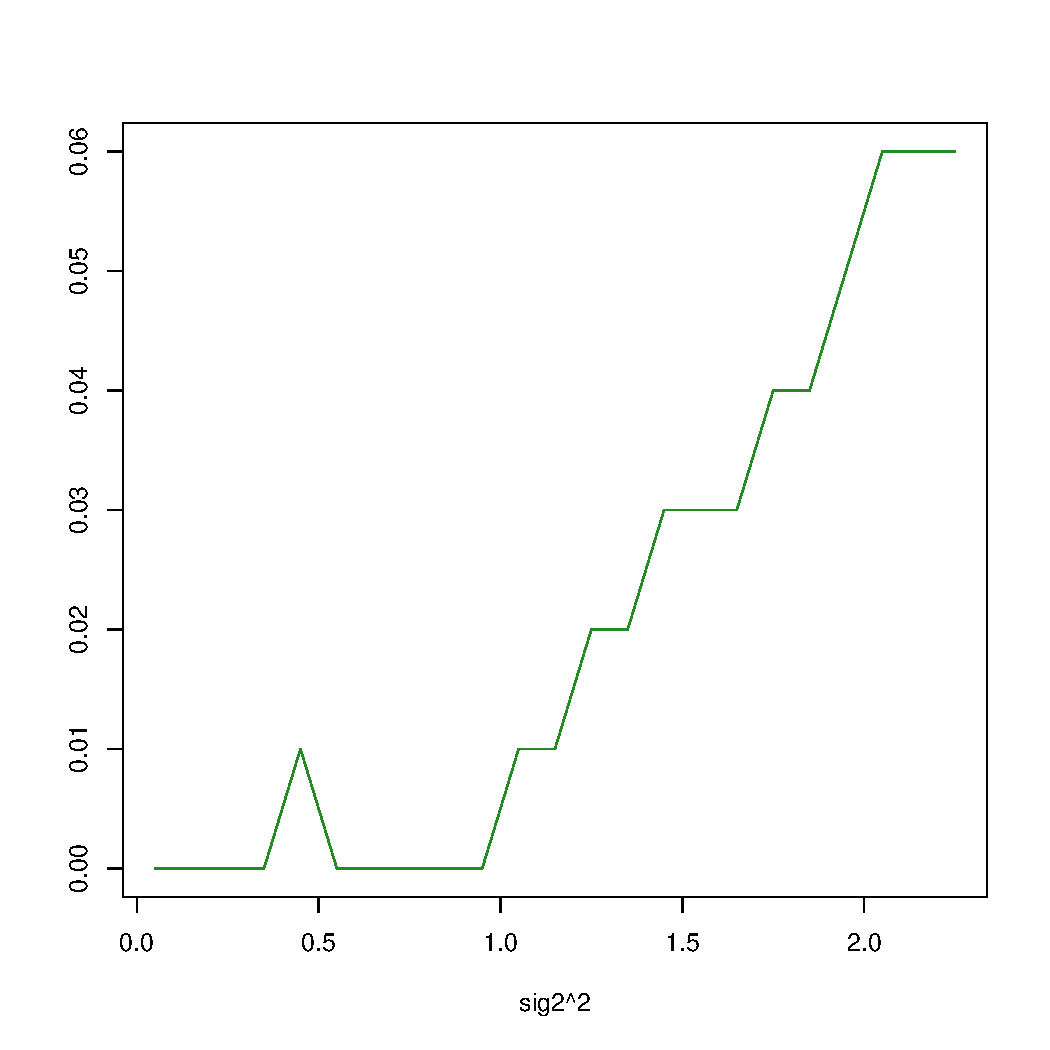
\includegraphics[width=1\linewidth]{gr_new_1.pdf}
				\caption{Ошибка аппроксимации медианы при $\sigma_{1}^{2} = 0.45$.} %% подпись к рисунку
				\label{ris7} %% метка рисунка для ссылки на него
			\end{minipage}
			\hfill
			\begin{minipage}[h]{0.4\linewidth}
				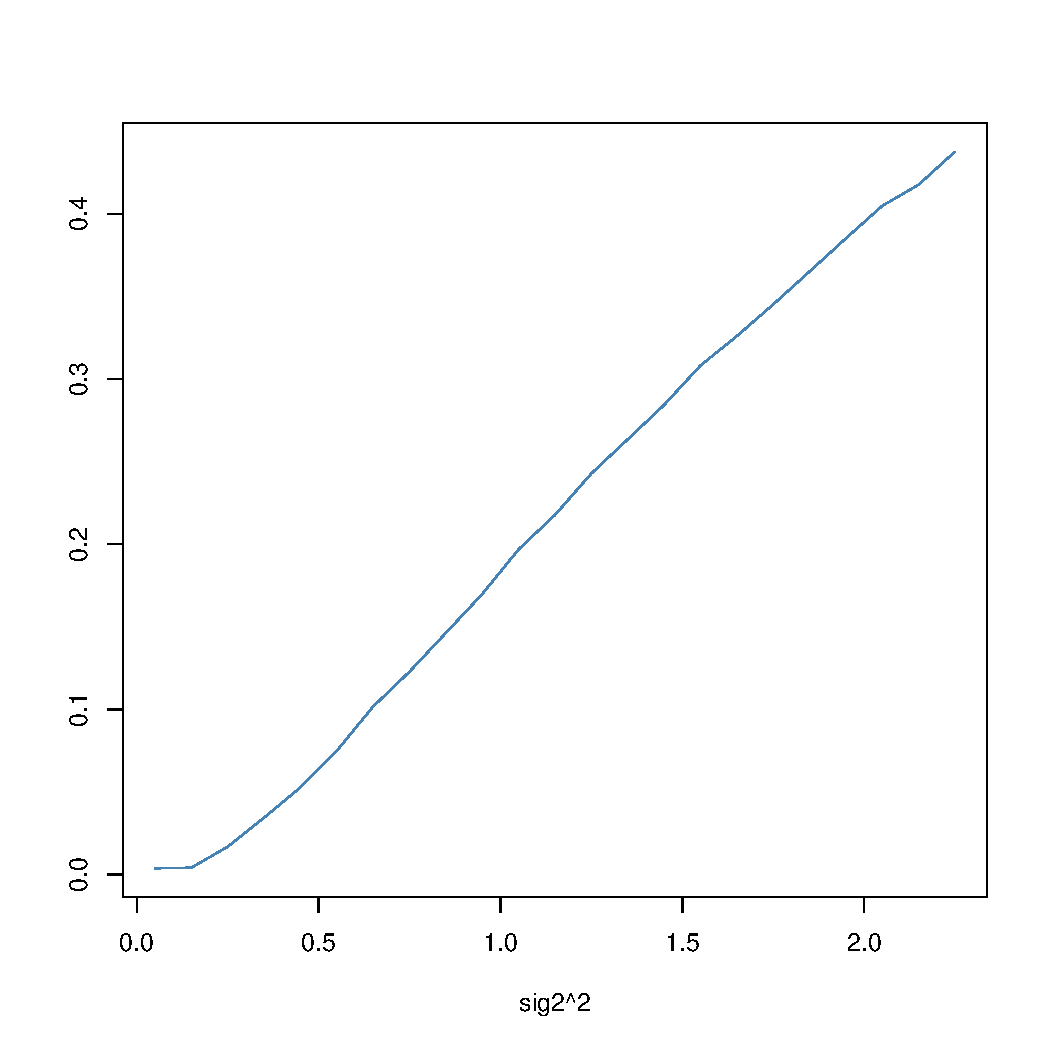
\includegraphics[width=1\linewidth]{gr_new_2.pdf}
				\caption{Ошибка аппроксимации $q_{10}$ при $\sigma_{1}^{2} = 0.45$.}
				\label{ris8}
			\end{minipage}
			\hfill
			\begin{minipage}[h]{0.4\linewidth}
				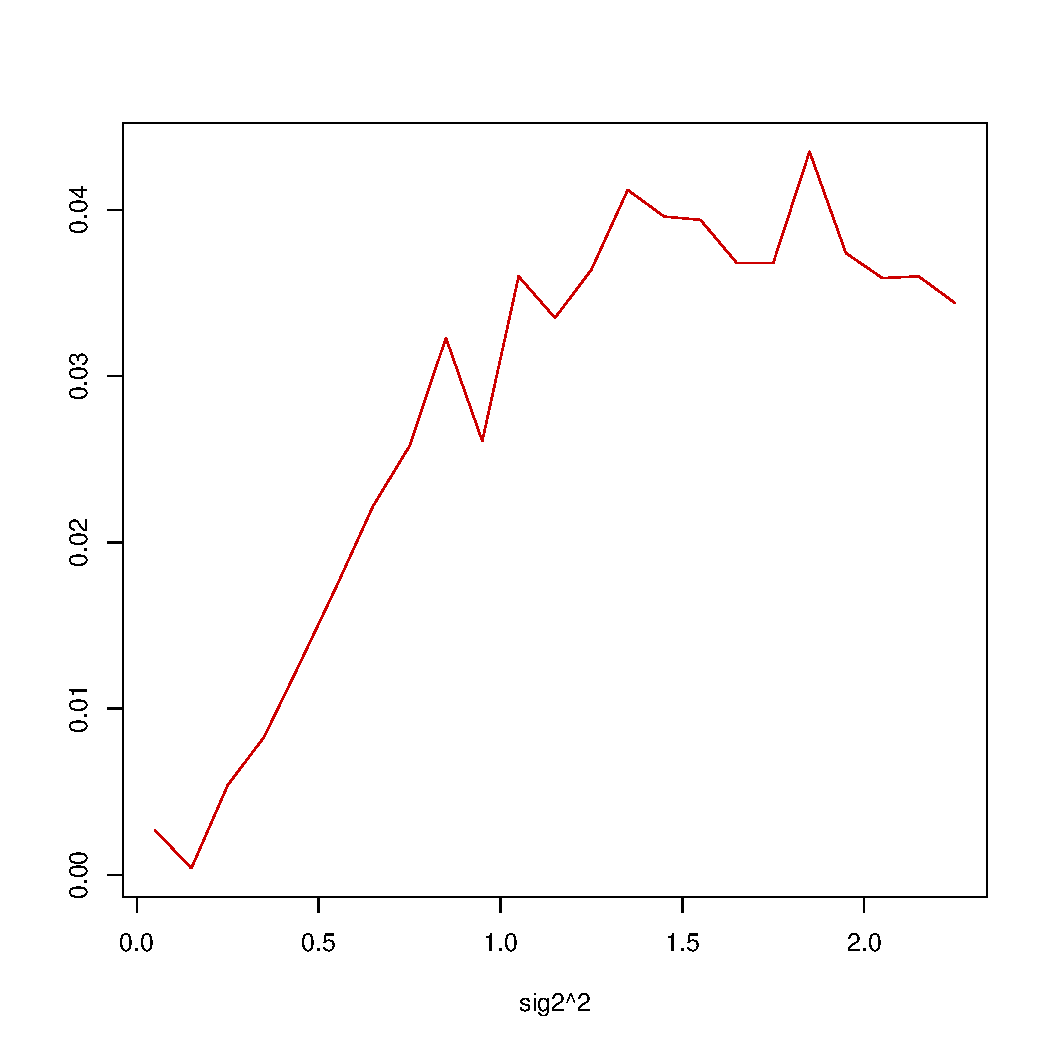
\includegraphics[width=1\linewidth]{gr_new_3.pdf}
				\caption{Ошибка аппроксимации $q_{90}$ при $\sigma_{1}^{2} = 0.45$.}
				\label{ris9}
			\end{minipage}
		\end{center}
	\end{figure}
	
	\begin{table}[!hhh]
		\centering
		\caption{$F_{\eta}(z_{50})$ в \% при 0.15 < $\sigma_{1}^{2}, \sigma_{2}^{2}$ < 2.25 }
		\label{tab4}
		\begin{tabular}{rrrrr}
			\hline
			& \textbf{0.15} & \textbf{0.85} & \textbf{1.55} & \textbf{2.25} \\
			\hline
			\textbf{0.15} & 0.51 & 0.50 & 0.49 & 0.48 \\ 
			\textbf{0.85} & 0.50 & 0.50 & 0.48 & 0.47 \\ 
			\textbf{1.55} & 0.49 & 0.50 & 0.48 & 0.46 \\ 
			\textbf{2.25} & 0.40 & 0.49 & 0.48 & 0.46 \\ 
			\hline
		\end{tabular}
	\end{table}
	
	\begin{table}[!hhh]
		\centering
		\caption{$F_{\eta}(z_{10})$ при 0.15 < $\sigma_{1}^{2}, \sigma_{2}^{2}$ < 2.25 }
		\label{tab5}
		\begin{tabular}{rrrrr}
			\hline
			& \textbf{0.15} & \textbf{0.85} & \textbf{1.55} & \textbf{2.25} \\
			\hline
			\textbf{0.15} & 0.09 & 0.06 & 0.04 & 0.02 \\ 
			\textbf{0.85} & 0.10 & 0.07 & 0.05 & 0.03 \\ 
			\textbf{1.55} & 0.05 & 0.08 & 0.06 & 0.04 \\ 
			\textbf{2.25} & 0.00 & 0.08 & 0.07 & 0.05 \\ 
			\hline
		\end{tabular}
	\end{table}
	
	\begin{table}[!hhh]
		\centering
		\caption{$F_{\eta}(z_{90})$ при 0.15 < $\sigma_{1}^{2}, \sigma_{2}^{2}$ < 2.25 }
		\label{tab6}
		\begin{tabular}{rrrrr}
			\hline
			& \textbf{0.15} & \textbf{0.85} & \textbf{1.55} & \textbf{2.25} \\
			\hline
			\textbf{0.15} & 0.90 & 0.90 & 0.90 & 0.90 \\ 
			\textbf{0.85} & 0.90 & 0.91 & 0.91 & 0.90 \\ 
			\textbf{1.55} & 0.93 & 0.90 & 0.91 & 0.91 \\ 
			\textbf{2.25} & 0.95 & 0.91 & 0.90 & 0.91 \\ 
			\hline
		\end{tabular}
	\end{table}
	
	Теперь посчитаем значения функции $F_{\eta}(x)$ от квантилей $z_{10}$, $z_{50}$, $z_{90}$ случайной величины $\eta_{n}$ при 0.15 < $\sigma_{1}^{2}, \sigma_{2}^{2}$ < 2.25. Результаты приведены в таблицаx \ref{tab4}, \ref{tab5} и \ref{tab6}.
	
	На графиках \ref{ris12} и \ref{ris13} представлены диаграммы с не очень большими ошибками квантилей. На графиках \ref{ris10} и \ref{ris11} наоборот с большими.
	
	\begin{figure}[!hhh]
		\begin{center}
			
			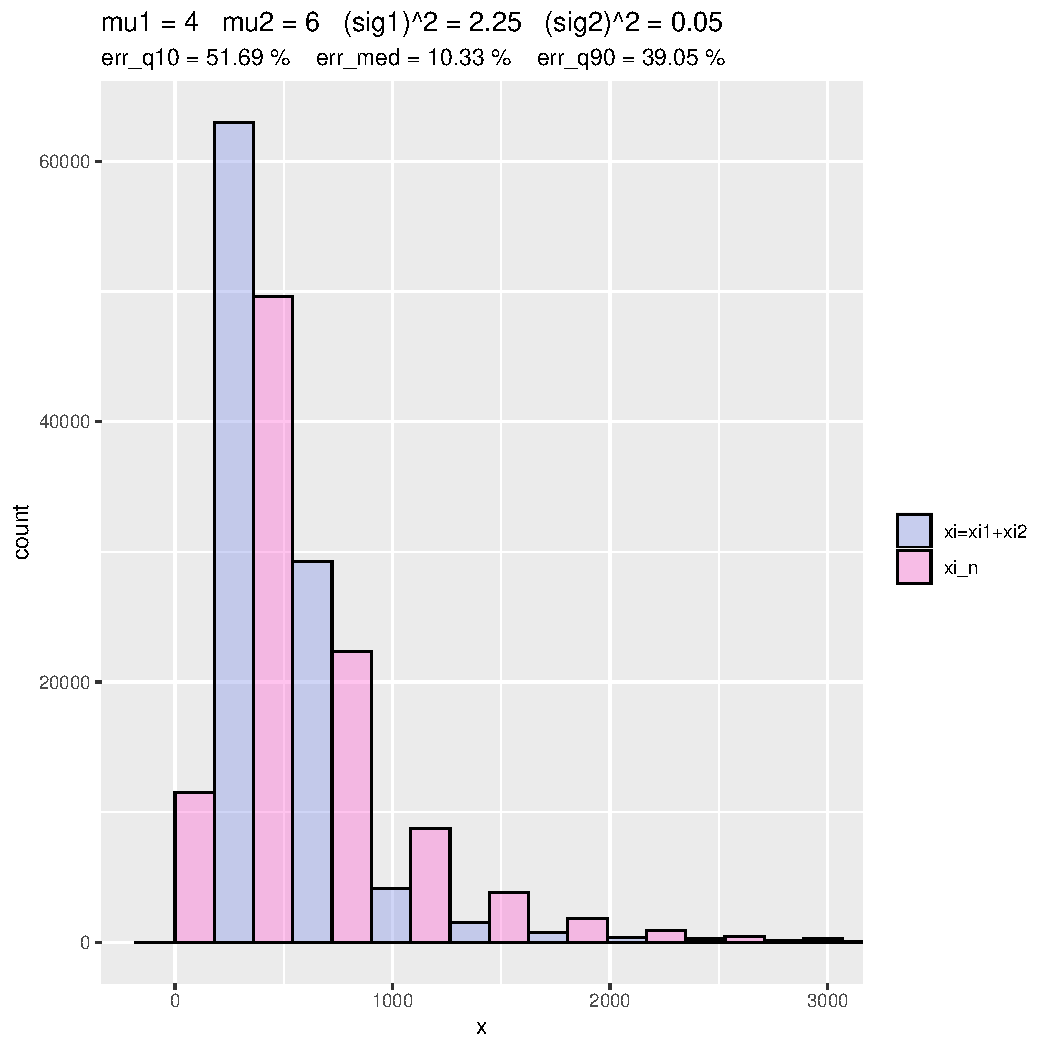
\includegraphics[width=1\linewidth]{hist_new_1.pdf}
			\caption{Сумма логнормальных} %% подпись к рисунку
			\label{ris10} %% метка рисунка для ссылки на него
			
		\end{center}
	\end{figure}
	
	\begin{figure}[!hhh]
		\begin{center}
			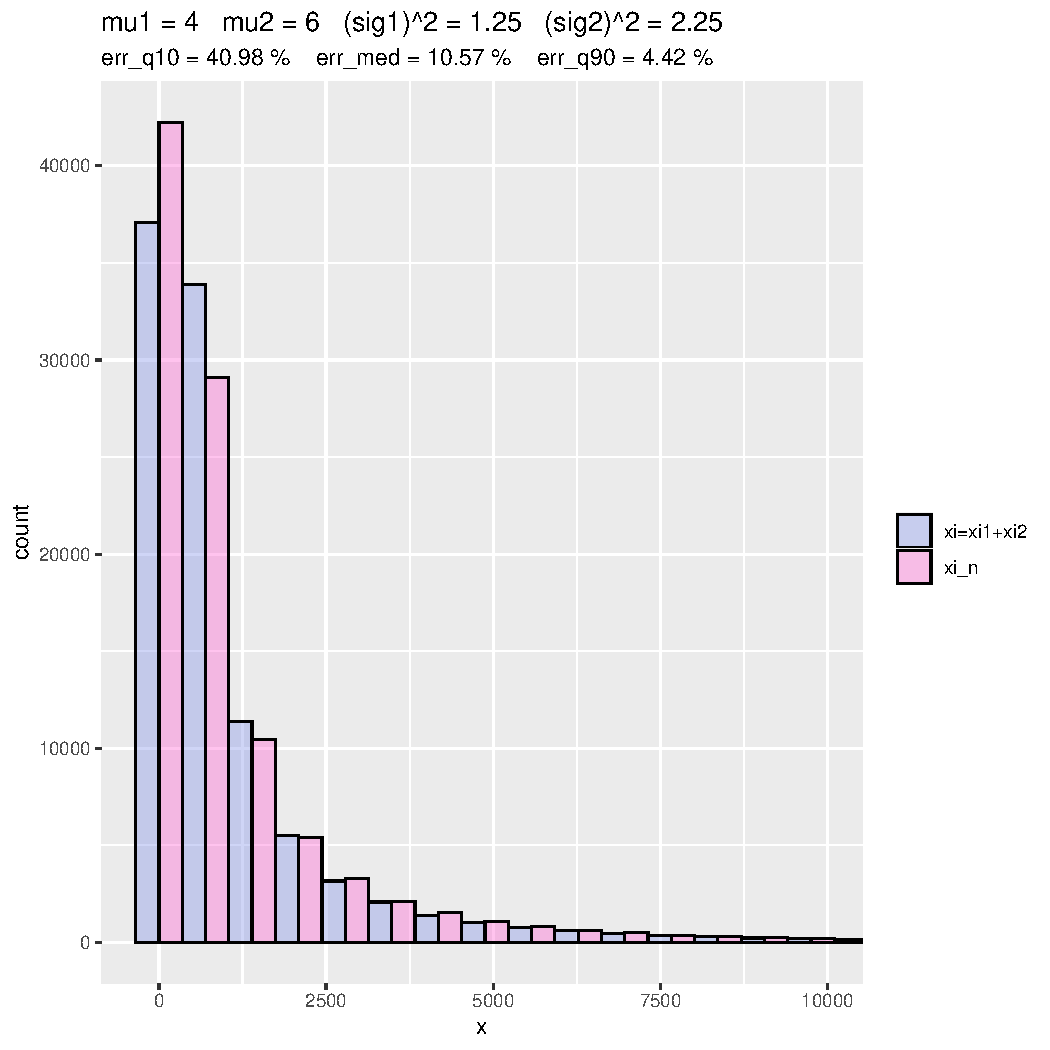
\includegraphics[width=1\linewidth]{hist_new_2.pdf}
			\caption{Сумма логнормальных}
			\label{ris11}
		\end{center}
	\end{figure}
	
	\begin{figure}[!hhh]
		\begin{center}
			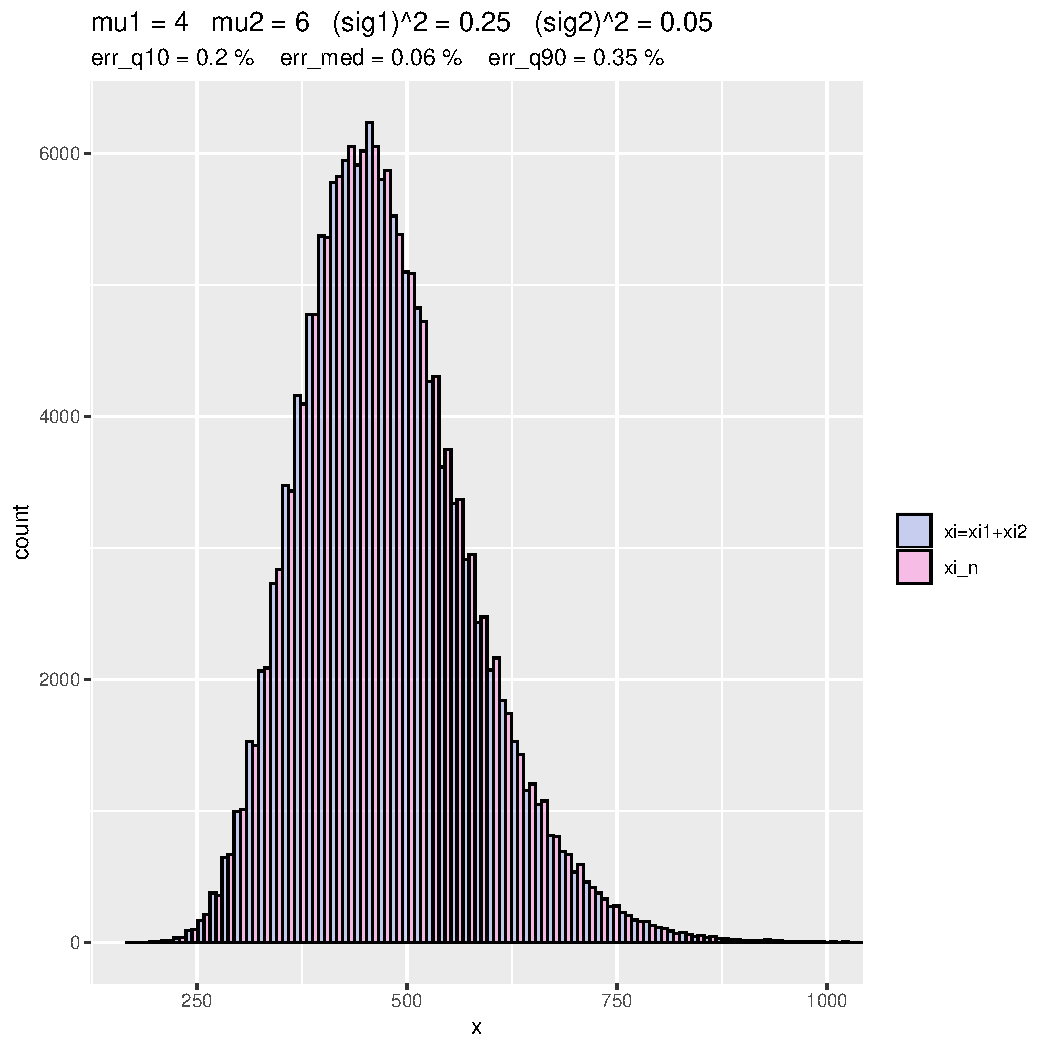
\includegraphics[width=1\linewidth]{hist_new_3.pdf}
			\caption{Сумма логнормальных}
			\label{ris12}
		\end{center}
	\end{figure}
	
	\begin{figure}[!hhh]
		\begin{center}
			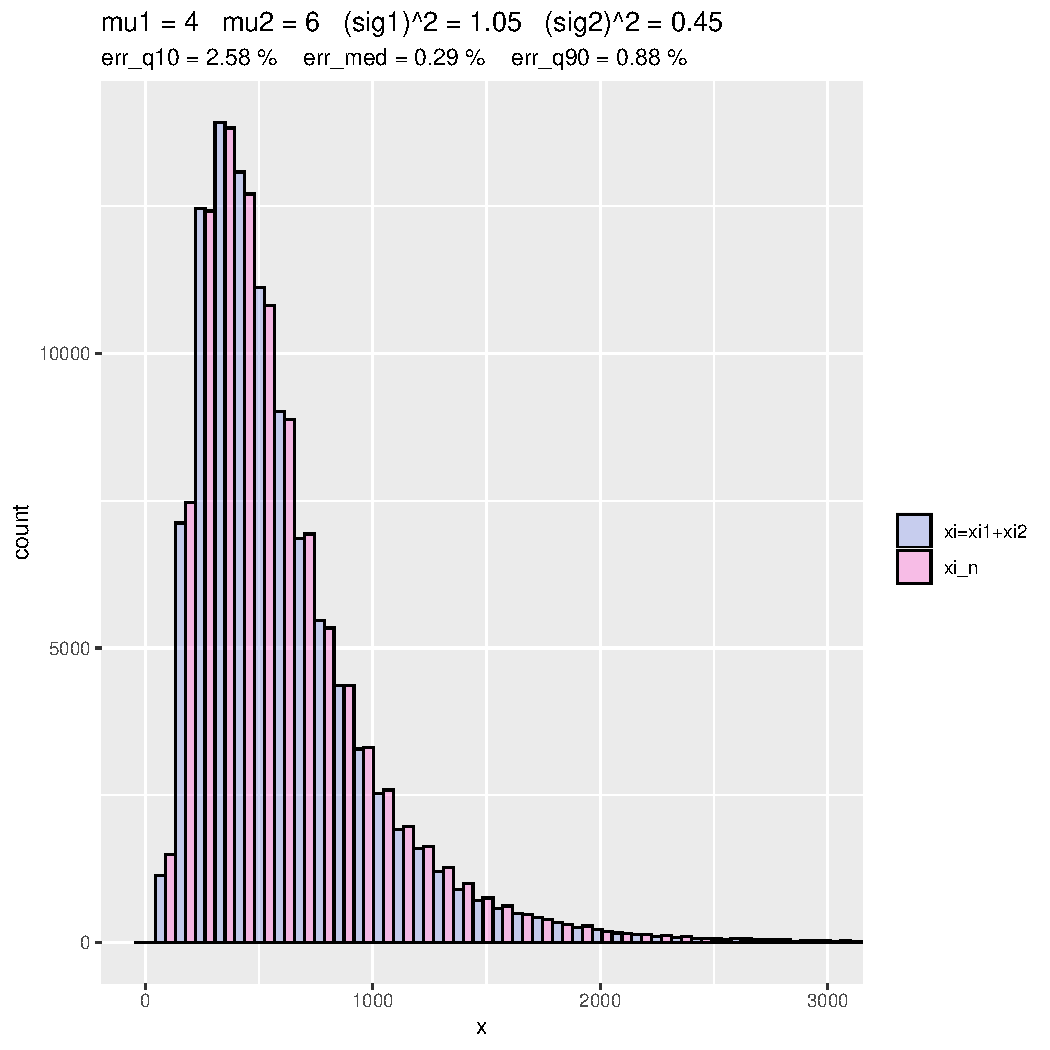
\includegraphics[width=1\linewidth]{hist_new_4.pdf}
			\caption{Сумма логнормальных}
			\label{ris13}
		\end{center}
	\end{figure}
	
	
	
	\section{Заключение}
	
	Таким образом, были получены следующие результаты: методы аппроксимации нормального и логнормального распределений, условие на $\sigma$ для аппроксимации логнормального распределения, точность аппроксимации логнормального правилом 30-40-30, методы аппроксимации суммы и произведения двух логнормальных распределений.
	
	При этом возникали проблемы с тем, что аппроксимировать дискретным распределением получается только при ограниченных значениях параметра $\sigma$ и тем, что для суммы логнормальных результат имеет ошибки, так как сумма логнормальных распределений не является логнормальным распределением.
	
	\addcontentsline{toc}{section}{ Список литературы}
	\begin{thebibliography}{1}
		\bibitem{Swansong} Keith G. Swanson's Swansong."--- Текст: электронный // stochastic: [сайт]."--- URL: https://www.stochastic.dk/post/swanson-s-swansong (дата обращения: 23.12.2021).
		
		\bibitem{Uncertainties} Uncertainties impacting reserves, revenue, and costs"--- Текст: электронный // AAPG Wiki: [сайт]."--- URL: https://wiki.aapg.org/Uncertainties impacting reserves, revenue, and costs (дата обращения: 27.05.2022).
		
		\bibitem{Discretization} Bickel, J. Eric, Lake, Larry W., and John Lehman. "Discretization, Simulation, and Swanson's (Inaccurate) Mean." SPE Econ Mgmt 3 (2011): 128–140. doi: https://doi.org/10.2118/148542-PA.
		
		\bibitem{Simulation} Bickel, J. Eric. "Discretization, Simulation, and the Value of Information." Paper presented at the SPE Annual Technical Conference and Exhibition, Denver, Colorado, USA, October 2011. doi: https://doi.org/10.2118/145690-MS.
		
		\bibitem{Performance} Moghadasi, Maryam and Jerry L. Jensen. “Performance Evaluation of Swanson’s Rule for the Case of Log-Normal Populations.” (2014). DOI:10.1007/978-3-642-32408.
		
		
	\end{thebibliography}
	
	\section{Приложение}
	
	На  С++ были реализованы следующие полезные на практике функции.
	
	$\bullet$ 
	
	Дано:
	значения квантилей $x_{\pi_{i}}$, математическое ожидание $m$, дисперсия $s^2$ непрерывной случайной величины.
	
	Задача:
	найти вероятности $p_{i}$ такие, что непрерывное распределение можно заменить дискретным с данными квантилями и полученными весами с сохранением математического ожидания и дисперсии.
	
	Решение описано в разделе 2.
	
	Система:
	
	\begin{equation*}
		\begin{pmatrix} 
			1&1&1\\ 
			x_{\pi_{1}} &  x_{\pi_{2}}  & x_{\pi_{3}} \\ 
			x_{\pi_{1}}^2~~&x_{\pi_{2}}^2  &x_{\pi_{3}}^2
		\end{pmatrix}
		\begin{pmatrix}p_{1}\\p_{2}\\ p_{3}\end{pmatrix}= \begin{pmatrix}1\\m\\m^{2}+s^{2}\end{pmatrix}.
	\end{equation*}
	
	Функция:
	
	vector<double> P (double $m$, double $s$, double $x_{\pi_{1}}$, double $x_{\pi_{2}}$, double $x_{\pi_{3}}$).
	
	
	$\bullet$
	
	Дано:
	вероятности $\pi_{i}$.
	
	Задача:
	найти вероятности $p_{i}$ для дискретного распределения, заменяющего исходное нормальное распределение, с любыми тремя квантилями $x_{\pi_{1}}$, $x_{\pi_{2}}$ и $x_{\pi_{3}}$.
	
	Решение описано в разделе 3.
	
	Система:
	
	\begin{equation*}
		\begin{pmatrix} 1&1&1\\ 
			\Phi^{-1}(\pi_{1})~~ &  \Phi ^{-1}(\pi_{2})~~  & \Phi ^{-1}(\pi_{3}) \\ 
			\Phi ^{-1}(\pi_{1})^{2}~~&\Phi ^{-1}(\pi_{2})^{2}~~  &\Phi ^{-1}(\pi_{3})^{2}
		\end{pmatrix}
		\begin{pmatrix}p_{1}\\p_{2}\\ p_{3}\end{pmatrix}= \begin{pmatrix}1\\0\\1\end{pmatrix}.
	\end{equation*}
	
	Функция:
	
	vector<double> PNormal (double $\pi_{1}$, double $\pi_{2}$, double $\pi_{3}$).
	
	$\bullet$
	
	Дано:
	вероятность $\pi$.
	
	Задача:
	найти вероятности $p_{i}$ для дискретного распределения, заменяющего исходное нормальное распределение, в случае симметричных квантилей вида  $\pi$, $0.5$ и $1-\pi$.
	
	Решение описано в разделе 3 с помощью системы \eqref{10}.
	
	Формулы:
	
	\begin{equation*}
		\begin{cases}
			p_{\pi} = \displaystyle{\dfrac{1}{2\Phi ^{-1}(\pi)^{2}}},\\ 
			p_{0.5}=\displaystyle{1-\dfrac{1}{\Phi ^{-1}(\pi)^{2}}} , \\ 
			p_{1-\pi}=\displaystyle{\dfrac{1}{2\Phi ^{-1}(\pi)^{2}}}.
		\end{cases}
	\end{equation*}
	
	Функция:
	
	vector<double> PNormalSim (double $\pi$).
	
	$\bullet$
	
	Дано:
	параметры нормального распределения $\mu$ и $\sigma$, соответствующего логнормальному распределению.
	
	Задача:
	найти параметры этого логнормального распределения $m$ и $s$. 
	
	Решение получено из определений логнормального распределения и соответствующего ему нормального распределения.
	
	Формулы:
	\begin{equation*}
		m = \exp(\mu+\frac{\sigma ^{2}}{2}),
	\end{equation*}
	\begin{equation*}
		s^{2} = m^{2}(\exp(\sigma^{2})-1).
	\end{equation*}
	
	Функции:
	
	double M (double $\mu$, double $\sigma$),
	
	double S (double $\mu$, double $\sigma$).
	
	$\bullet$
	
	Дано:
	вероятности $\pi_{1}$, $\pi_{2}$, значения квантилей $x_{\pi_{1}}$, $x_{\pi_{2}}$.
	
	Задача:
	найти дисперсию логарифмически нормального распределения через квантили дискретного распределения, которое его заменяет.
	
	Решение описано в разделе 4.2, получена формула \eqref{11}.
	
	Формула:
	\begin{equation*}
		\displaystyle{\sigma = \dfrac{\log\left(\dfrac{x_{\pi_{2}}}{x_{\pi_{1}}}\right)}{\Phi ^{-1}(\pi_{2}) - \Phi ^{-1}(\pi_{1})}}.
	\end{equation*}
	
	Функция:
	
	double Sig (double $\pi_{1}$, double $\pi_{2}$, double $x_{\pi_{1}}$, double $x_{\pi_{2}}$).
	
	$\bullet$
	
	Дано:
	вероятность $\pi$, значения квантилей $x_{\pi}$, $x_{0.5}$.
	
	Задача:
	найти дисперсию логарифмически нормального распределения через квантили дискретного распределения, которое его заменяет в случае симметричных кванилей.
	
	Решение получено как частый случай формулы \eqref{11}.
	
	Формула:
	\begin{equation*}
		\sigma=\frac{\ln(x_{\pi})-\ln(x_{0.5})}{\Phi^{-1}(\pi)}.
	\end{equation*}
	
	Функция:
	
	double SigSim (double $\pi$, double $x_{\pi}$, double $x_{0.5}$).
	
	
	$\bullet$
	
	Дано:
	вероятность $\pi$, параметры нормального распределения $\mu$, $\sigma$.
	
	Задача:
	найти квантили логнормальной случайной величины, зная параметры соответствующего нормального распределения в случае симметричных квантилей. 
	
	Решение описано в разделе 5.
	
	Формулы:
	\begin{equation*}
		\ln(x_{\pi})=\mu+\Phi^{-1}(\pi)\sigma,
	\end{equation*}
	\begin{equation*}
		\ln(x_{0.5})=\mu,
	\end{equation*}
	\begin{equation*}
		\ln(x_{1-\pi})=\mu+\Phi^{-1}(1-\pi)\sigma.
	\end{equation*}
	
	Функция:
	
	double lnX (double $\pi$, double $\mu$, double $\sigma$).
	
	$\bullet$
	
	Дано:
	вероятность $\pi$, дисперсии $\sigma_{1}$ и $\sigma_{2}$ нормальных случайных величин.
	
	Задача:
	понять, какой квантиль получается при перемножении квантилей логнормальных случайных величин, через дисперсии соответствующих нормальных случайных величин в случае симметричных квантилей.
	
	Решение описано в разделе 5.
	
	Формулы:
	
	\begin{equation*}
		\mathsf{P}(\xi_{1}\xi_{2}< x_{\pi}y_{\pi}) = \Phi\left(\frac{\Phi^{-1}(\pi)(\sigma_{1}+\sigma_{2})}{\sqrt{\sigma_{1}^{2}+\sigma_{2}^{2}}}\right),
	\end{equation*}
	
	\begin{equation*}
		q =\frac{\Phi^{-1}(\pi)(\sigma_{1}+\sigma_{2})}{\sqrt{\sigma_{1}^{2}+\sigma_{2}^{2}}}.
	\end{equation*}
	
	Функция:
	
	double ProbPr (double $\pi$, double $\sigma_{1}$, double $\sigma_{2}$).
	
	$\bullet$
	
	Дано:
	вероятность $\pi$, квантили $x_{\pi}$, $x_{0.5}$ и $y_{\pi}$, $y_{0.5}$.
	
	Задача:
	понять, какой квантиль получается при перемножении $\pi$-ых квантилей логнормальных случайных величин, через логарифмы $\pi$-го и $0.5$-го квантилей.
	
	Решение описано в разделе 5, получена формула \eqref{18}.
	
	Формулы:
	
	\begin{equation*}
		\mathsf{P}(\xi_{1}\xi_{2}< x_{\pi}y_{\pi}) =\Phi\left(\frac{\Phi^{-1}(\pi)(\ln(x_{0.5})+\ln(y_{0.5})-\ln(x_{\pi})-\ln(y_{\pi}))}{\sqrt{(\ln(x_{0.5})-\ln(x_{\pi}))^{2}+(\ln(y_{0.5})-\ln(y_{\pi}))^{2}}}\right),
	\end{equation*}
	
	\begin{equation*}
		q =\frac{\Phi^{-1}(\pi)(\ln(x_{0.5})+\ln(y_{0.5})-\ln(x_{\pi})-\ln(y_{\pi}))}{\sqrt{(\ln(x_{0.5})-\ln(x_{\pi}))^{2}+(\ln(y_{0.5})-\ln(y_{\pi}))^{2}}}.
	\end{equation*}
	
	Функция:
	
	double ProbPrX (double $\pi$, double $x_{\pi}$, double $x_{0.5}$, double $y_{\pi}$, double $y_{0.5}$).
	
	
	$\bullet$
	
	Дано:
	вероятность $\pi$, квантили $x_{\pi}$, $x_{0.5}$ и $y_{\pi}$, $y_{0.5}$.
	
	Задача:
	найти значения $\pi$-го квантиля для произведения двух логнормально распределенных случайных величин через их квантили.
	
	Решение описано в разделе 7.
	
	Формулы:
	
	\begin{equation*}
		z_{\pi}=\exp\left(\dfrac{\ln(x_{\pi}y_{\pi})-\ln(x_{0.5}y_{0.5})}{q}\Phi^{-1}(\pi)+\ln(x_{0.5}y_{0.5})\right),
	\end{equation*}
	
	\begin{equation*}
		q=\Phi^{-1}(\mathsf{P}(\xi_{1}\xi_{2}< x_{\pi}y_{\pi})).
	\end{equation*}
	
	Функция:
	
	double Q (double $\pi$, double $x_{\pi}$, double $x_{0.5}$, double $y_{\pi}$, double $y_{0.5}$).
	
	
	
\end{document}